\chapter{Результаты работы}

В данной главе приводятся результаты настоящей диссертационной работы. Описывается верификация разработанной модели процесса сухого электронно-лучевого травления резиста, а также ее применение для определения предельного разрешения метода СЭЛТР и контраста получаемого изображения. Помимо этого, разработанная модель используется для исследования влияния флуктуаций параметров процесса СЭЛТР на конечный профиль линии, получаемой этим методом, а также для определения параметров, обеспечивающих формирование методом СЭЛТР синусоидальных голографических решеток.

\section{Верификация модели сухого электронно-лучевого травления резиста} \label{sec:verification}

Для верификации разработанной модели методом СЭЛТР были получены периодические структуры в слое ПММА на кремниевой подложке. Как и в более ранних экспериментах, использовался резист PMMA 950K A2 от компании <<Allresist>>, начальная толщина слоя ПММА составляла 500 нм. Экспонирование производилось в камере растрового электронного микроскопа CAMSCAN~S-4, который был модифицирован для возможности нагрева образца. Давление в камере микроскопа поддерживалось на уровне 10$^\text{-5}$ мбар, энергия электронного пучка составляла 20 кэВ, диаметр пучка -- около 600 нм.

Экспонирование резиста производилось ``в кадр'', размеры кадра составляли 2.4$\times$1.9~мм$^\text{2}$, число линий в кадре равнялось 625. Ток экспонирования $I$ находился в диапазоне 4.56--5.62 нА, время экспонирования $t_\mathrm{exp}$ варьировалось от 100 до 200 с, таким образом, доза экспонирования на единицу длины линии $D_\mathrm{l}$ составляла 3.00--7.38 нКл/см. Температура образцов при экспонировании $T$ варьировалась от 130 до 150~$^\circ$C, скорость охлаждения подложки после экспонирования составляла около 0.2~$^\circ$C/с (экспериментальная кривая охлаждения приведена на рисунке~\ref{fig:exp_cooling}). Профили линий были получены методом атомно-силовой микроскопии с использованием микроскопа Nanopics 2100.

\begin{figure}[h!]
	\begin{center}
		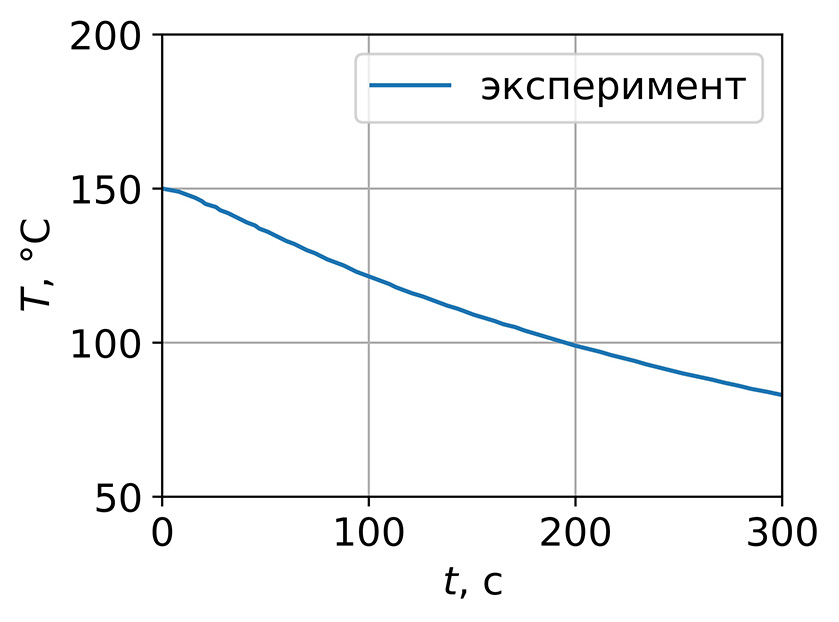
\includegraphics[width=0.5\linewidth]{DEBER_verification/cooling_FINAL_200} \\
	\end{center}
	\vspace{-1em}
	\caption{Экспериментальная зависимость температуры подложки образца от времени при охлаждении после экспонирования.}
	\label{fig:exp_cooling}
	\vspace{1em}
\end{figure}

Полученные в эксперименте профили были промоделированы с использованием алгоритма, описанного в разделе~\ref{sec:DEBER_model} (рисунок~\ref{fig:DEBER_3D_sim}).
Для снижения требуемого машинного времени моделирование проводилось для участка одной линии длиной 100 нм, влияние соседних линий учитывалось за счет использования периодических граничных условий.
Число разрывов молекул ПММА, локальная среднечисловая молекулярная масса ПММА и объемы микрополостей вычислялись для ячеек размерами 100$\times$100$\times$5 нм$\ppp$ (по осям $X$, $Y$ и $Z$, соответственно).

\begin{figure}[h!]
	\begin{center}
		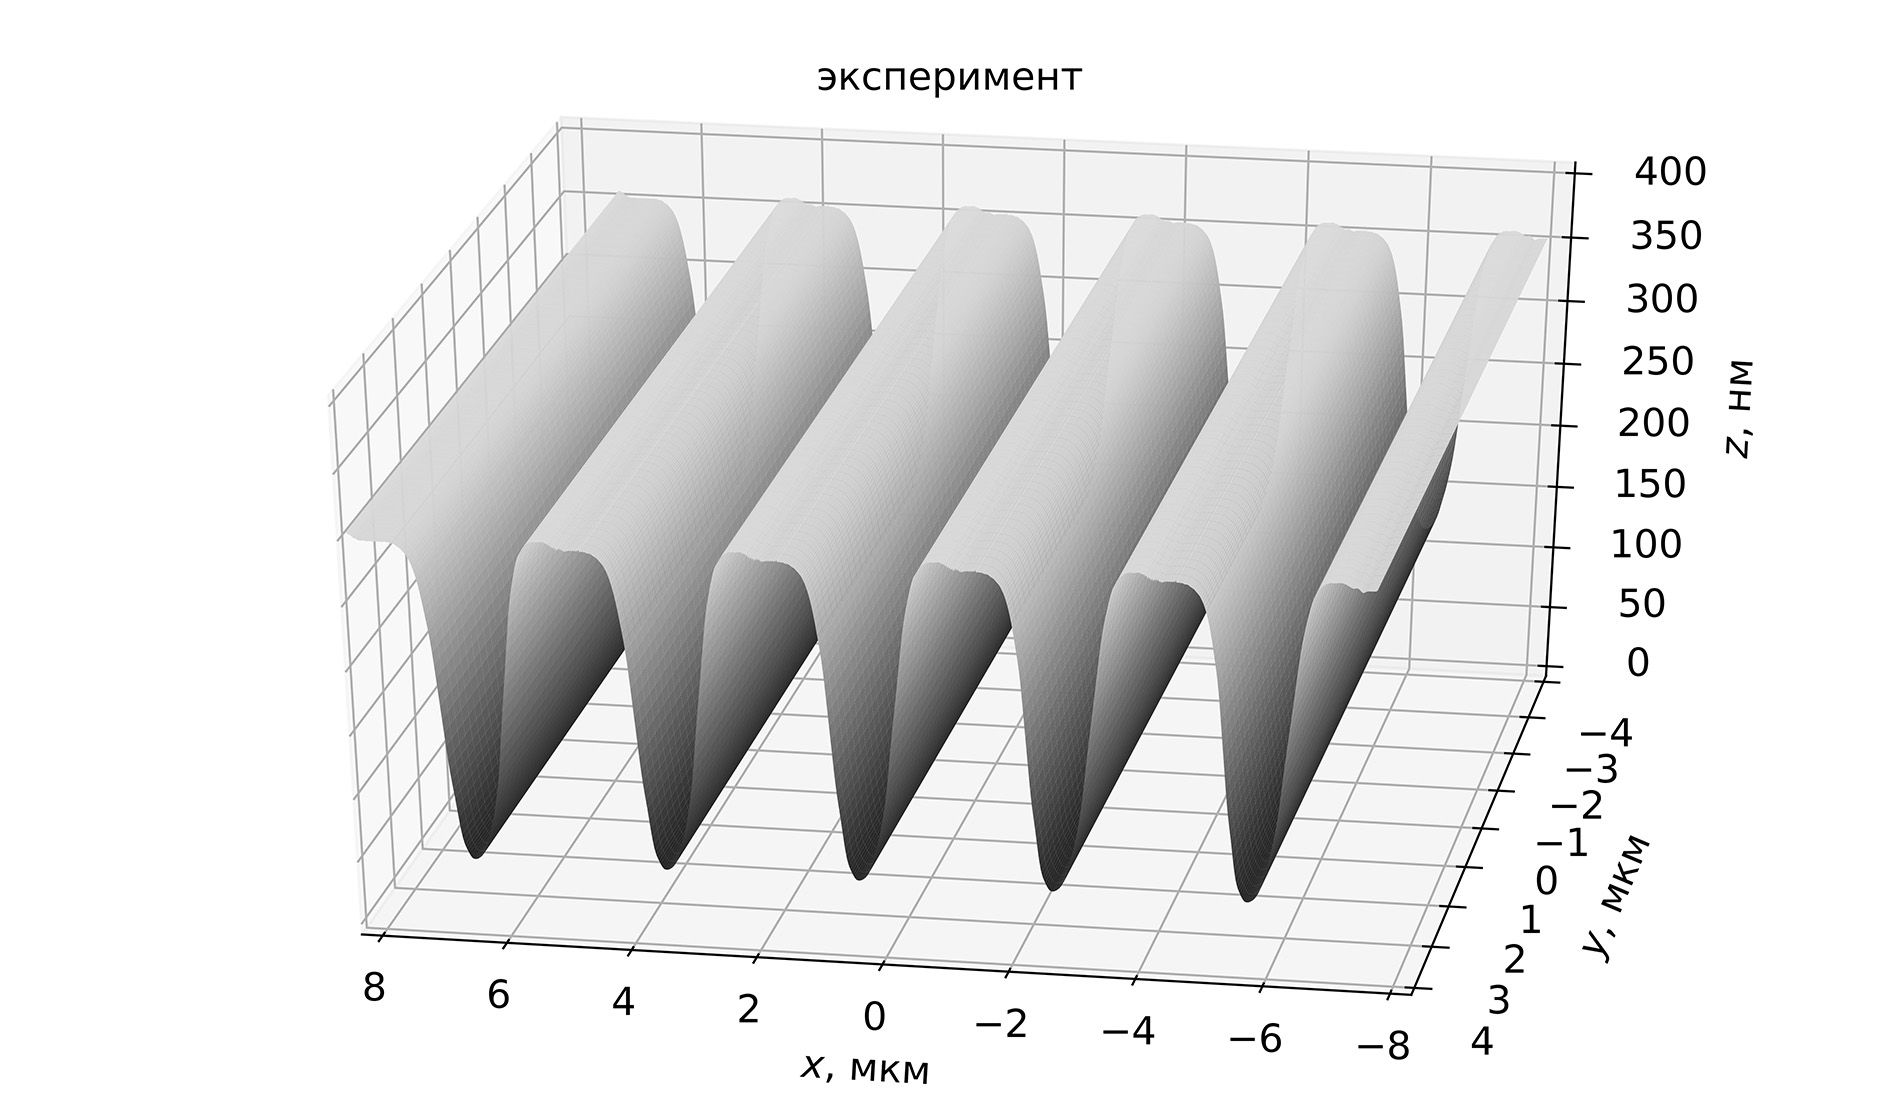
\includegraphics[width=\linewidth]{DEBER_verification/366_EXP_2_50_title_200} \\
		\vspace{-10.7em} \text{\hspace{-25em} a)} \vspace{9.7em} \\
		\vspace{-1em}
		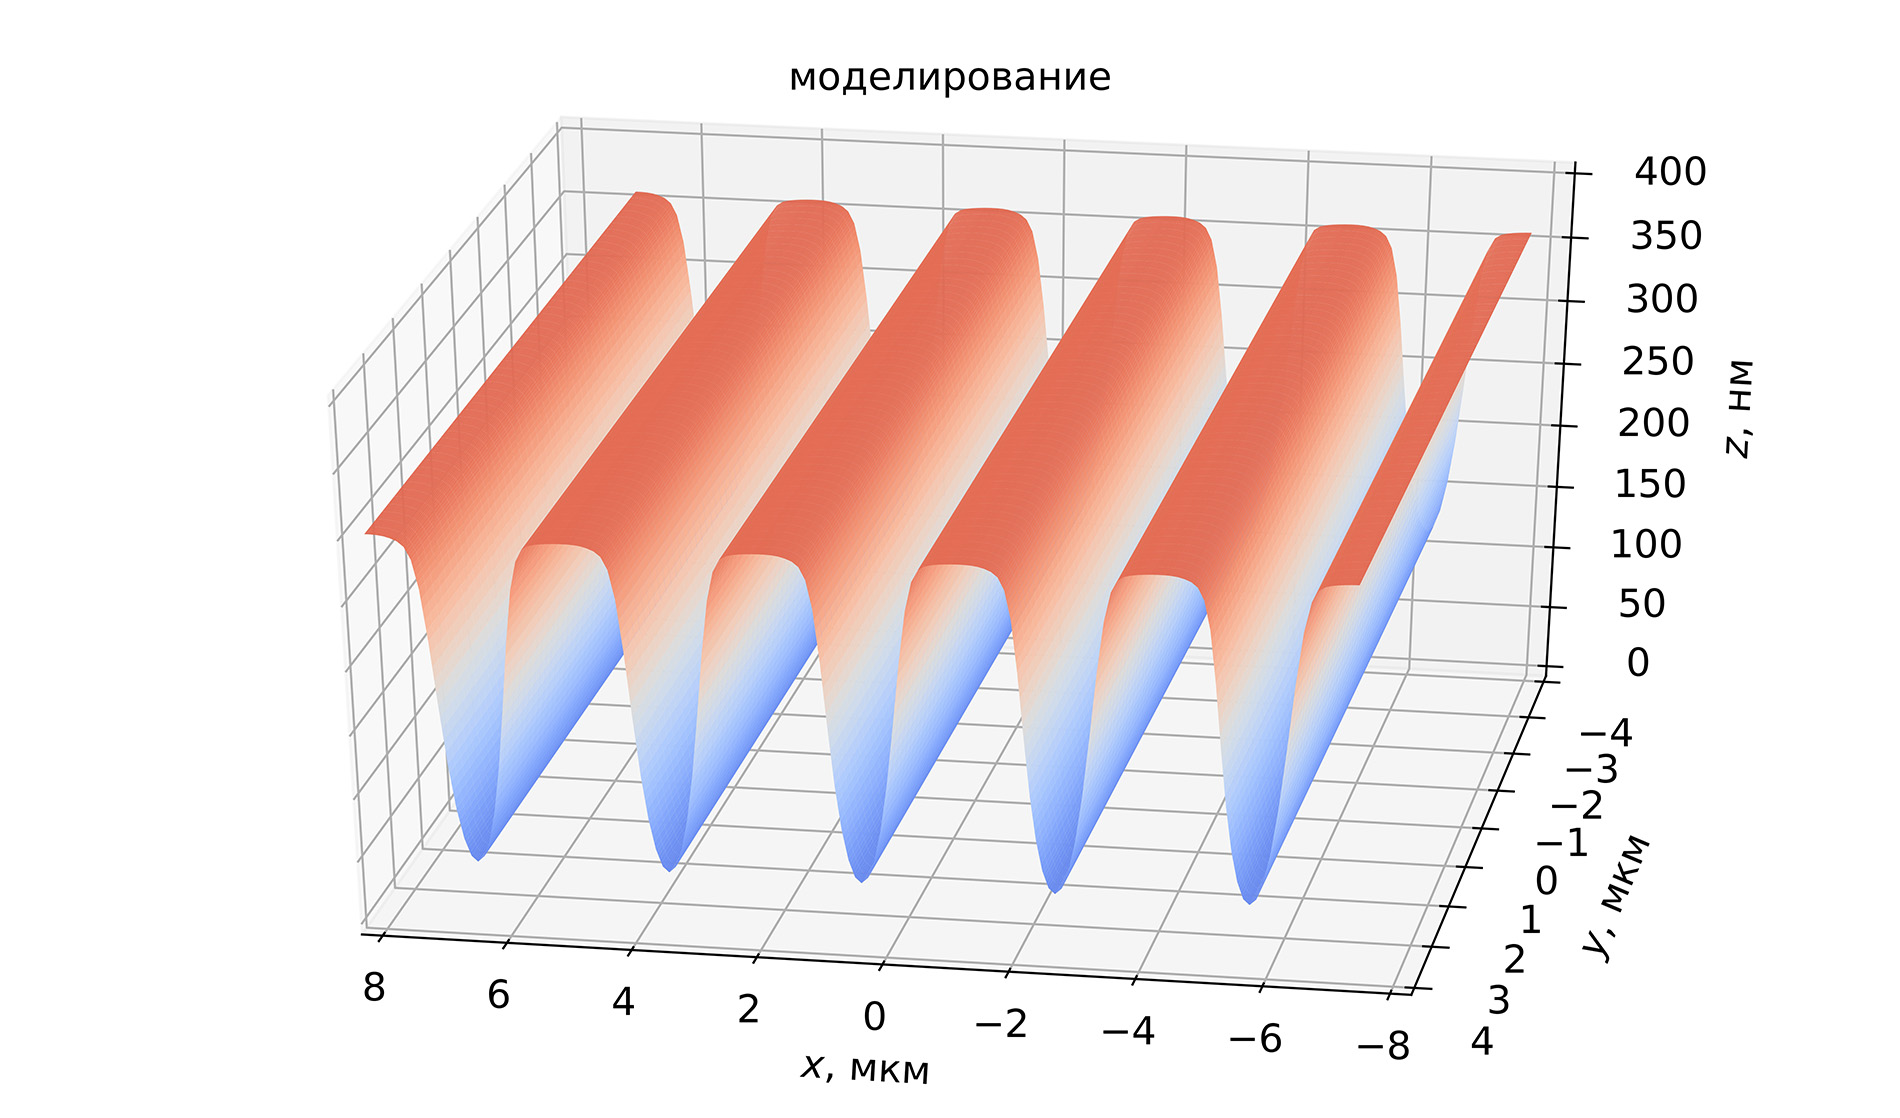
\includegraphics[width=\linewidth]{DEBER_verification/366_SIM_50_2_title_200} \\
		\vspace{-10.7em} \text{\hspace{-25em} б)} \vspace{10.7em} \\
	\end{center}
	\vspace{-2em}
	\caption{Трехмерное изображение поверхности структуры, полученной методом СЭЛТР при $T$ = 150~$^\circ$C, $t_\mathrm{exp}$ = 100 c, $I$ = 4.56 нА (a) и поверхности, полученной при моделировании (б).}
	\label{fig:DEBER_3D_sim}
\end{figure}

Для учета стохастической природы алгоритма моделирования для каждого из экспериментальных профилей проводилось 100 независимых моделирований и на основе профилей, полученных в отдельных моделированиях, рассчитывался усредненный промоделированный профиль.
Здесь и далее термином ``промоделированный профиль'' будет обозначаться профиль, полученный именно таким образом.
Сравнение экспериментальных и промоделированных профилей приведено на рисунке~\ref{fig:DEBER_4_profiles}.
Высокая степень воспроизведения экспериментальных профилей указывает на достоверность разработанной модели процесса СЭЛТР.
Было также установлено, что при описанных выше параметрах экспонирования средняя длина кинетической цепи при деполимеризации ПММА остается постоянной на протяжении первых 100 с процесса, и ее значения составляют 100 и 150 для температур 130 и 150~$^\circ$C соответственно.
При дальнейшем экспонировании средняя длина кинетической цепи снижается, и на временном промежутке 100-200 с ее значения составляют 30 и 70 для температур 130 и 150~$^\circ$C соответственно.

\begin{figure}[h!]
	\begin{minipage}{0.48\textwidth}
		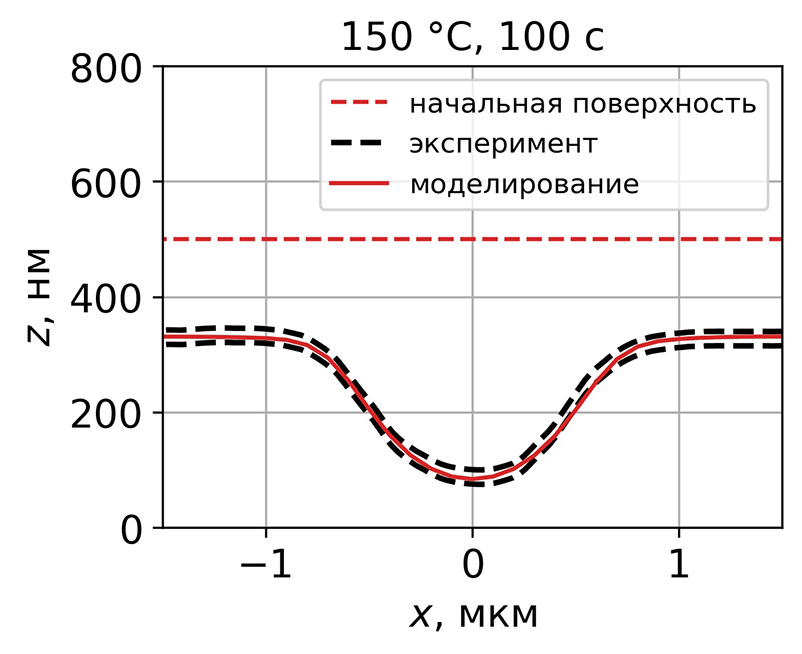
\includegraphics[width=\linewidth]{DEBER_verification/150C_100s_14_FINAL_200} \\
		\vspace{-13em} \\ \text{\hspace{0em} a}) \\ \vspace{13em}
	\end{minipage}
	\begin{minipage}{0.48\textwidth}
		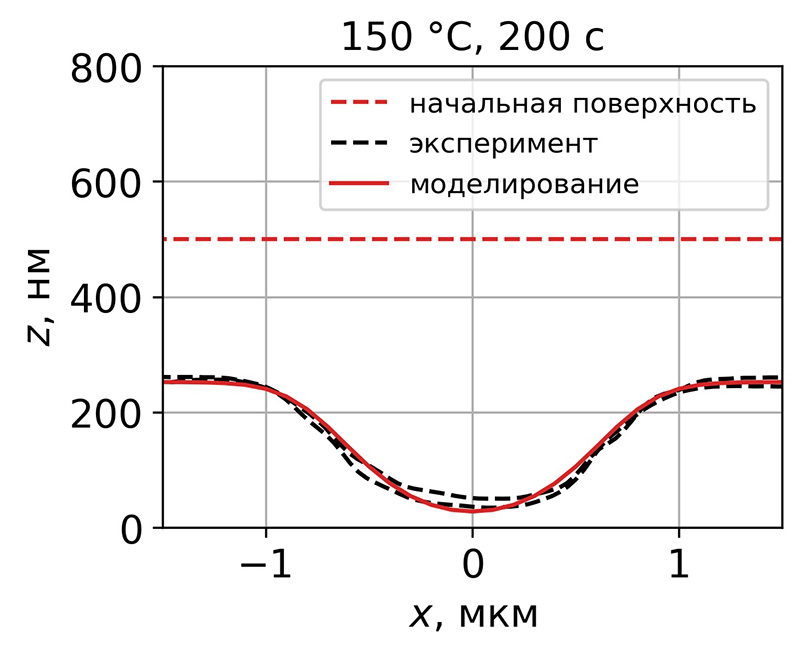
\includegraphics[width=\linewidth]{DEBER_verification/150C_200s_14_FINAL_200} \\
		\vspace{-13em} \\ \text{\hspace{-0.1em} б}) \\ \vspace{13em}
	\end{minipage}

	\vspace{-3em}

	\begin{minipage}{0.48\textwidth}
		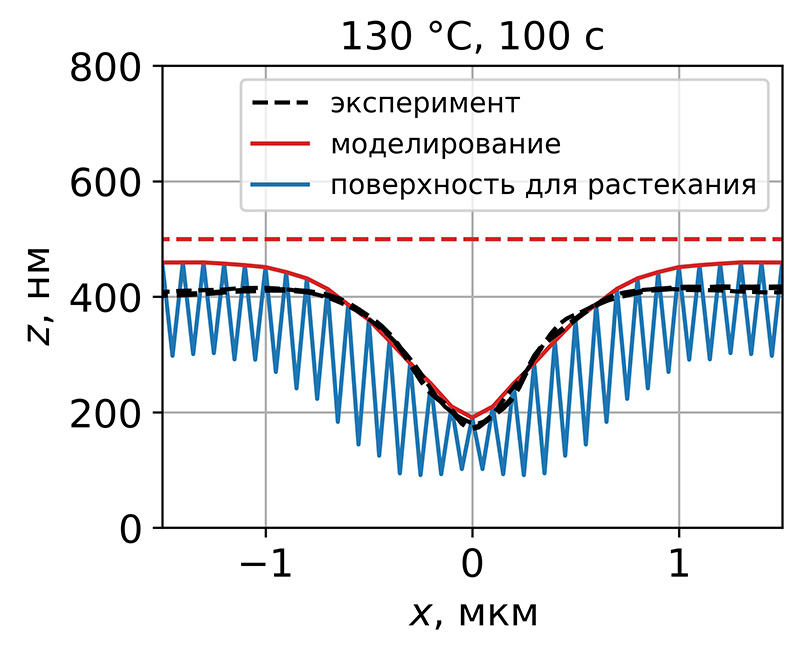
\includegraphics[width=\linewidth]{DEBER_verification/130C_100s_14_FINAL_200} \\
		\vspace{-13em} \\ \text{\hspace{0em} в}) \\ \vspace{13em}
	\end{minipage}
	\begin{minipage}{0.48\textwidth}
		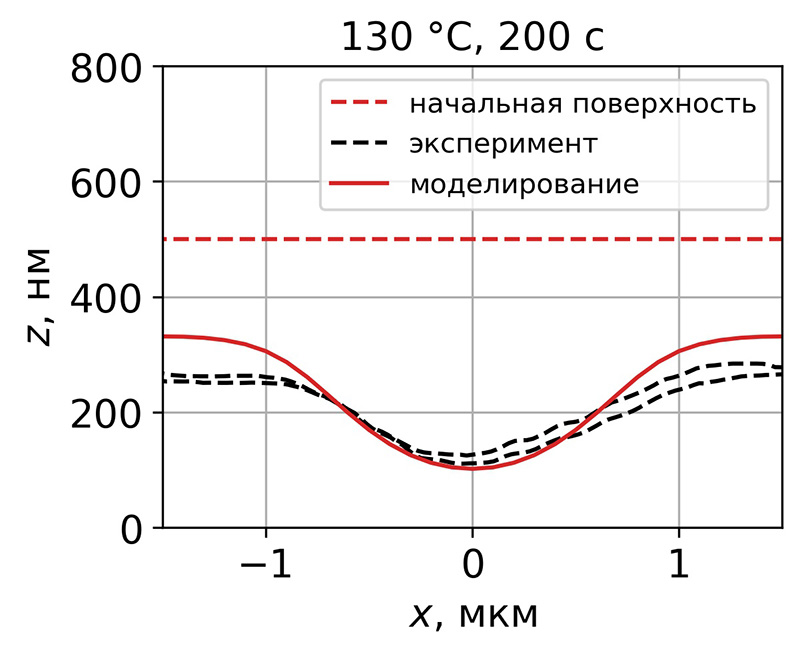
\includegraphics[width=\linewidth]{DEBER_verification/130C_200s_14_FINAL_200} \\
		\vspace{-13em} \\ \text{\hspace{-0.1em} г}) \\ \vspace{13em}
	\end{minipage}
	\vspace{-3em}
	\caption{
		Верификация разработанной модели процесс СЭЛТР -- сравнение экспериментальных и промоделированных профилей для следующих условий экспонирования: a) $T$ = 150~$^\circ$C, $t_\mathrm{exp}$ = 100 c, $D_\mathrm{l}$ = 3.00 нКл/см; б) $T$ = 150~$^\circ$C, $t_\mathrm{exp}$ = 200 c, $D_\mathrm{l}$ = 6.73 нКл/см; в) $T$ = 130~$^\circ$C, $t_\mathrm{exp}$ = 100 c, $D_l$ = 3.12 нКл/см; \linebreak г) $T$ = 130~$^\circ$C, $t_\mathrm{exp}$ = 200 c, $D_\mathrm{l}$ = 7.38 нКл/см.
		Во всех случаях начальная энергия электронного пучка составляла 20 кэВ, диаметр пучка -- около 600~нм, охлаждение описывалось кривой, приведенной на рисунке~\ref{fig:exp_cooling}.
		Черная пунктирная линия обозначает профили, полученные в эксперименте, красная пунктирная линия -- начальное положение поверхности ПММА, синяя линия -- пилообразную поверхность, использовавшуюся для моделирования растекания слоя ПММА со внутренними микрополостями.}
	\label{fig:DEBER_4_profiles}
	\vspace{1em}
\end{figure}

На рисунке~\ref{fig:DEBER_sigmas} приведены зависимости среднеквадратичного отклонения точек промоделированных профилей от $x$-координаты, полученные на основе 100 отдельно промоделированных профилей для каждого набора параметров экспонирования.
Из рисунка видно, что для профилей, полученных при полном заполнении микрополостей внутри слоя ПММА на момент остывания образца, среднеквадратичное отклонение точек профиля составляет от 0.5 до 3~нм со средним значением около 2 нм.
Однако, при наличии микрополостей внутри слоя ПММА на момент остывания (образец, приведенный на рисунке~\ref{fig:DEBER_4_profiles}в) среднеквадратичное отклонение точек профиля в центре линии превышает 10~нм.

\begin{figure}[t]
	\begin{center}
		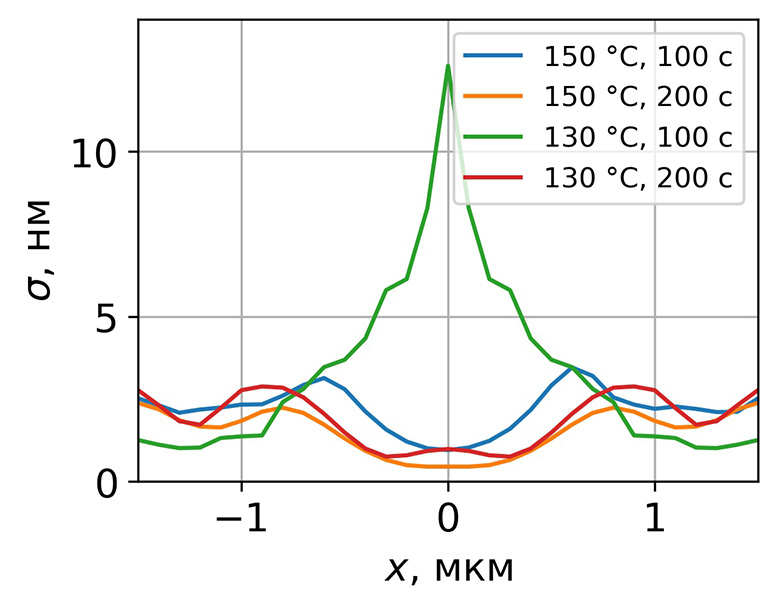
\includegraphics[width=0.5\linewidth]{DEBER_verification/DEBER_sigmas_FINAL_200}
	\end{center}
	\vspace{-1em}
	\caption{Зависимости среднеквадратичного отклонения точек промоделированных профилей от $x$-координаты, полученные для каждого набора параметров экспонирования.}
	\label{fig:DEBER_sigmas}
	\vspace{1em}
\end{figure}

\section{Предельное разрешение метода сухого электронно-лучевого травления резиста}

Исследование экспериментальных профилей показало, что при использовании пучка диаметром около 600 нм латеральное разрешение метода СЭЛТР, которое может быть оценено как ширина профиля на половине от максимальной глубины, составляет около 1 мкм. На основе разработанной модели процесса СЭЛТР можно предложить два пути увеличения разрешения данного метода.

Во-первых, латеральное разрешение метода СЭЛТР может быть увеличено за счет использования узкого высокоэнергетического пучка. Малый диаметр пучка позволит локализовать большинство разрывов молекул ПММА в центре линии, что вызовет интенсивную деполимеризацию, образование мономера и снижение вязкости резиста в этой области. В свою очередь, за счет высокой энергии пучка будет снижено число разрывов на краях линии, вызванных обратно отраженными электронами. При этом будет необходимо подобрать время экспонирования так, чтобы на момент остывания образца микрополости в центре линии оказались заполненными, а микрополости на краях -- остались незаполненными. Во-вторых, использование узкого низкоэнергетического пучка также может увеличить латеральное разрешение. При низкой энергии первичных электронов все разрывы полимерных молекул будут происходить вблизи центра линии за счет относительно небольшой глубины проникновения электронов. В этом случае микрополости будут формироваться только в ограниченной области вблизи центра линии, что исключит ``проседание'' краев линии.

Промоделированные профили, полученные методом методом СЭЛТР с латеральным разрешением, увеличенным обоими вышеописанными способами, приведены на рисунке~\ref{fig:DEBER_resolution}. При моделировании диаметр пучка был принят равным 10 нм, температура образцов -- 150~$^\circ$C/с, начальная толщина слоя ПММА -- 500 нм. Энергия пучка составляла 25 кэВ (высокоэнергетический пучок) и 5 кэВ (низкоэнергетический пучок), скорость охлаждения образцов -- 10~$^\circ$C/с. Моделирование проводилось для экспонирования вдоль одиночной линии, плотность тока экспонирования на единицу длины линии составляла 30 пА/см.

\begin{figure}[t]
	\begin{minipage}{0.48\textwidth}
		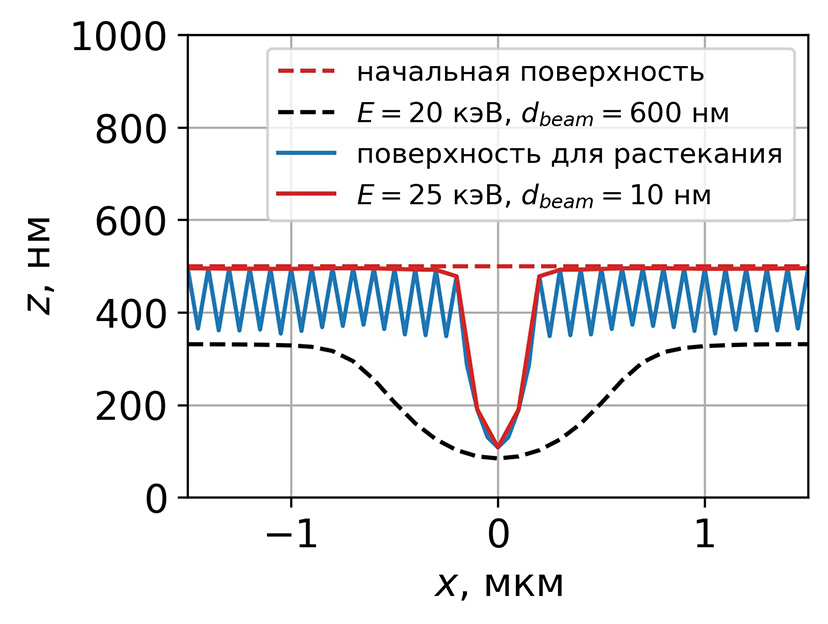
\includegraphics[width=\linewidth]{DEBER_resolution/resolution_25_um_200} \\
		\vspace{-28.7ex} \\ \text{\hspace{0em} a}) \\ \vspace{28.7ex}
	\end{minipage}
	\begin{minipage}{0.48\textwidth}
		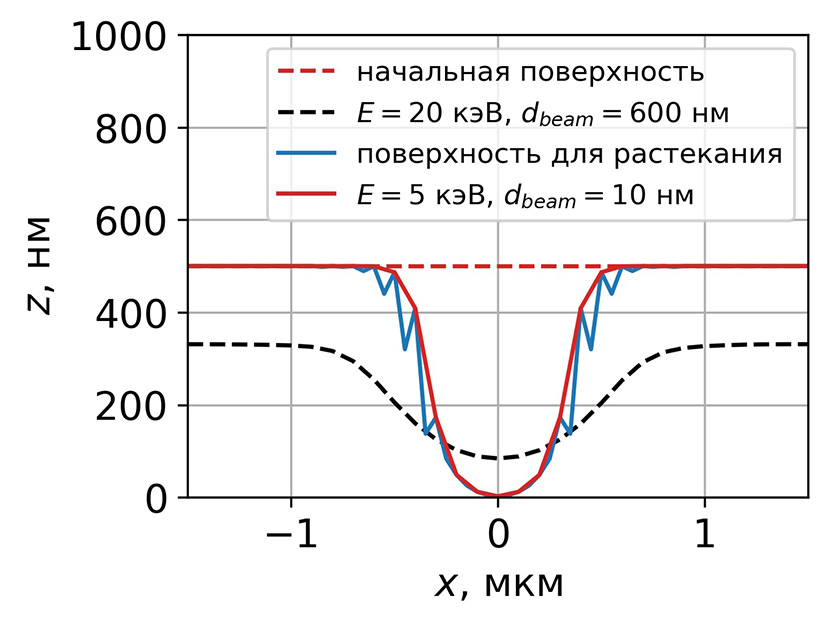
\includegraphics[width=\linewidth]{DEBER_resolution/resolution_5_um_200} \\
		\vspace{-28.7ex} \\ \text{\hspace{-0.1em} б}) \\ \vspace{28.7ex}
	\end{minipage}
	\vspace{-3.5em}
	\caption{Моделирование линий, полученных методом СЭЛТР с использованием узкого высокоэнергетического (25 кэВ, а)) и низкоэнергетического (5 кэВ, б)) пучка. Диаметр пучка составляет 10 нм, температура образцов -- 150~$^\circ$C/с, начальная толщина слоя ПММА -- 500 нм. Экспонирование производилось ``в линию'', плотность тока на единицу длины линии составляла 30 пА/см, скорость охлаждения образцов -- 10~$^\circ$C/с.}
	\label{fig:DEBER_resolution}
\end{figure}

Исходя из результатов моделирования, можно заключить, что использование узкого высокоэнергетического пучка способно обеспечить латеральное разрешение метода СЭЛТР до 300 нм. Было также установлено, что в этом случае толщина слоя ПММА в центре линии ограничена снизу значением около 100 нм, причиной чего является относительно большая средняя длина свободного пробега электронов при высоких энергиях, а также быстрое заполнение линии близлежащим резистом за счет процессов растекания. Использование узкого низкоэнергетического пучка, в свою очередь, обеспечивает латеральное разрешение всего лишь около 600 нм, однако, делает возможным полное травление резиста в центре линии за счет относительно небольшой средней длины свободного пробега электронов при низких энергиях. Следует также отметить, что во втором случае профиль полученной линии будет более устойчив к процессам растекания после экспонирования, поскольку вязкость резиста на краях линии будет оставаться практически на начальном уровне.

При этом в обоих вышеописанных случаях угол наклона профиля на полувысоте составляет около 70$^\circ$, что практически в три раза превышает максимальное значение угла наклона профиля в экспериментальных структурах \linebreak (около 25~$^\circ$).

\section{Влияние флуктуаций параметров экспонирования на результирующий профиль}

Разработанная модель СЭЛТР позволяет исследовать влияние параметров процесса на профиль линии, получаемой методом СЭЛТР.
В том числе эта модель может использоваться для исследования влияния флуктуаций параметров экспонирования на результирующий профиль линии.
Как и ранее, считалось, что экспонирование резиста в процессе СЭЛТР производится \linebreak ``в кадр'' с параметрами кадра, описанными в разделе~\ref{sec:verification}.
В качестве исходных параметров экспонирования были приняты $E$ = 20 кэВ, $T$ = 150~$^\circ$C, $t_\mathrm{exp}$ = 100 c и \linebreak $I$ = 4.56 нА, диаметр пучка составлял 600 нм, начальная толщина слоя ПММА -- 500 нм, зависимость температуры образца от времени при его охлаждении описывалась экспериментальной кривой охлаждения, приведенной на рисунке~\ref{fig:exp_cooling} (профиль линии, получаемой при этих параметрах процесса СЭЛТР, приведен на рисунке~\ref{fig:DEBER_4_profiles}a).
Поскольку в этом случае в резисте на момент остывания отсутствуют микрополости, среднеквадратичное отклонение точек промоделированных профилей было принято равным 2 нм (рисунок~\ref{fig:DEBER_sigmas}).
Далее определялись значения параметров экспонирования (энергии пучка, тока экспонирования и температуры образца), при которых отклонения точек промоделированного профиля от исходного были сопоставимы со среднеквадратичным отклонением при моделировании (рисунки~\ref{fig:DEBER_vary_E}, \ref{fig:DEBER_vary_I} и \ref{fig:DEBER_vary_T}).

\begin{figure}[h!]
	\begin{center}
		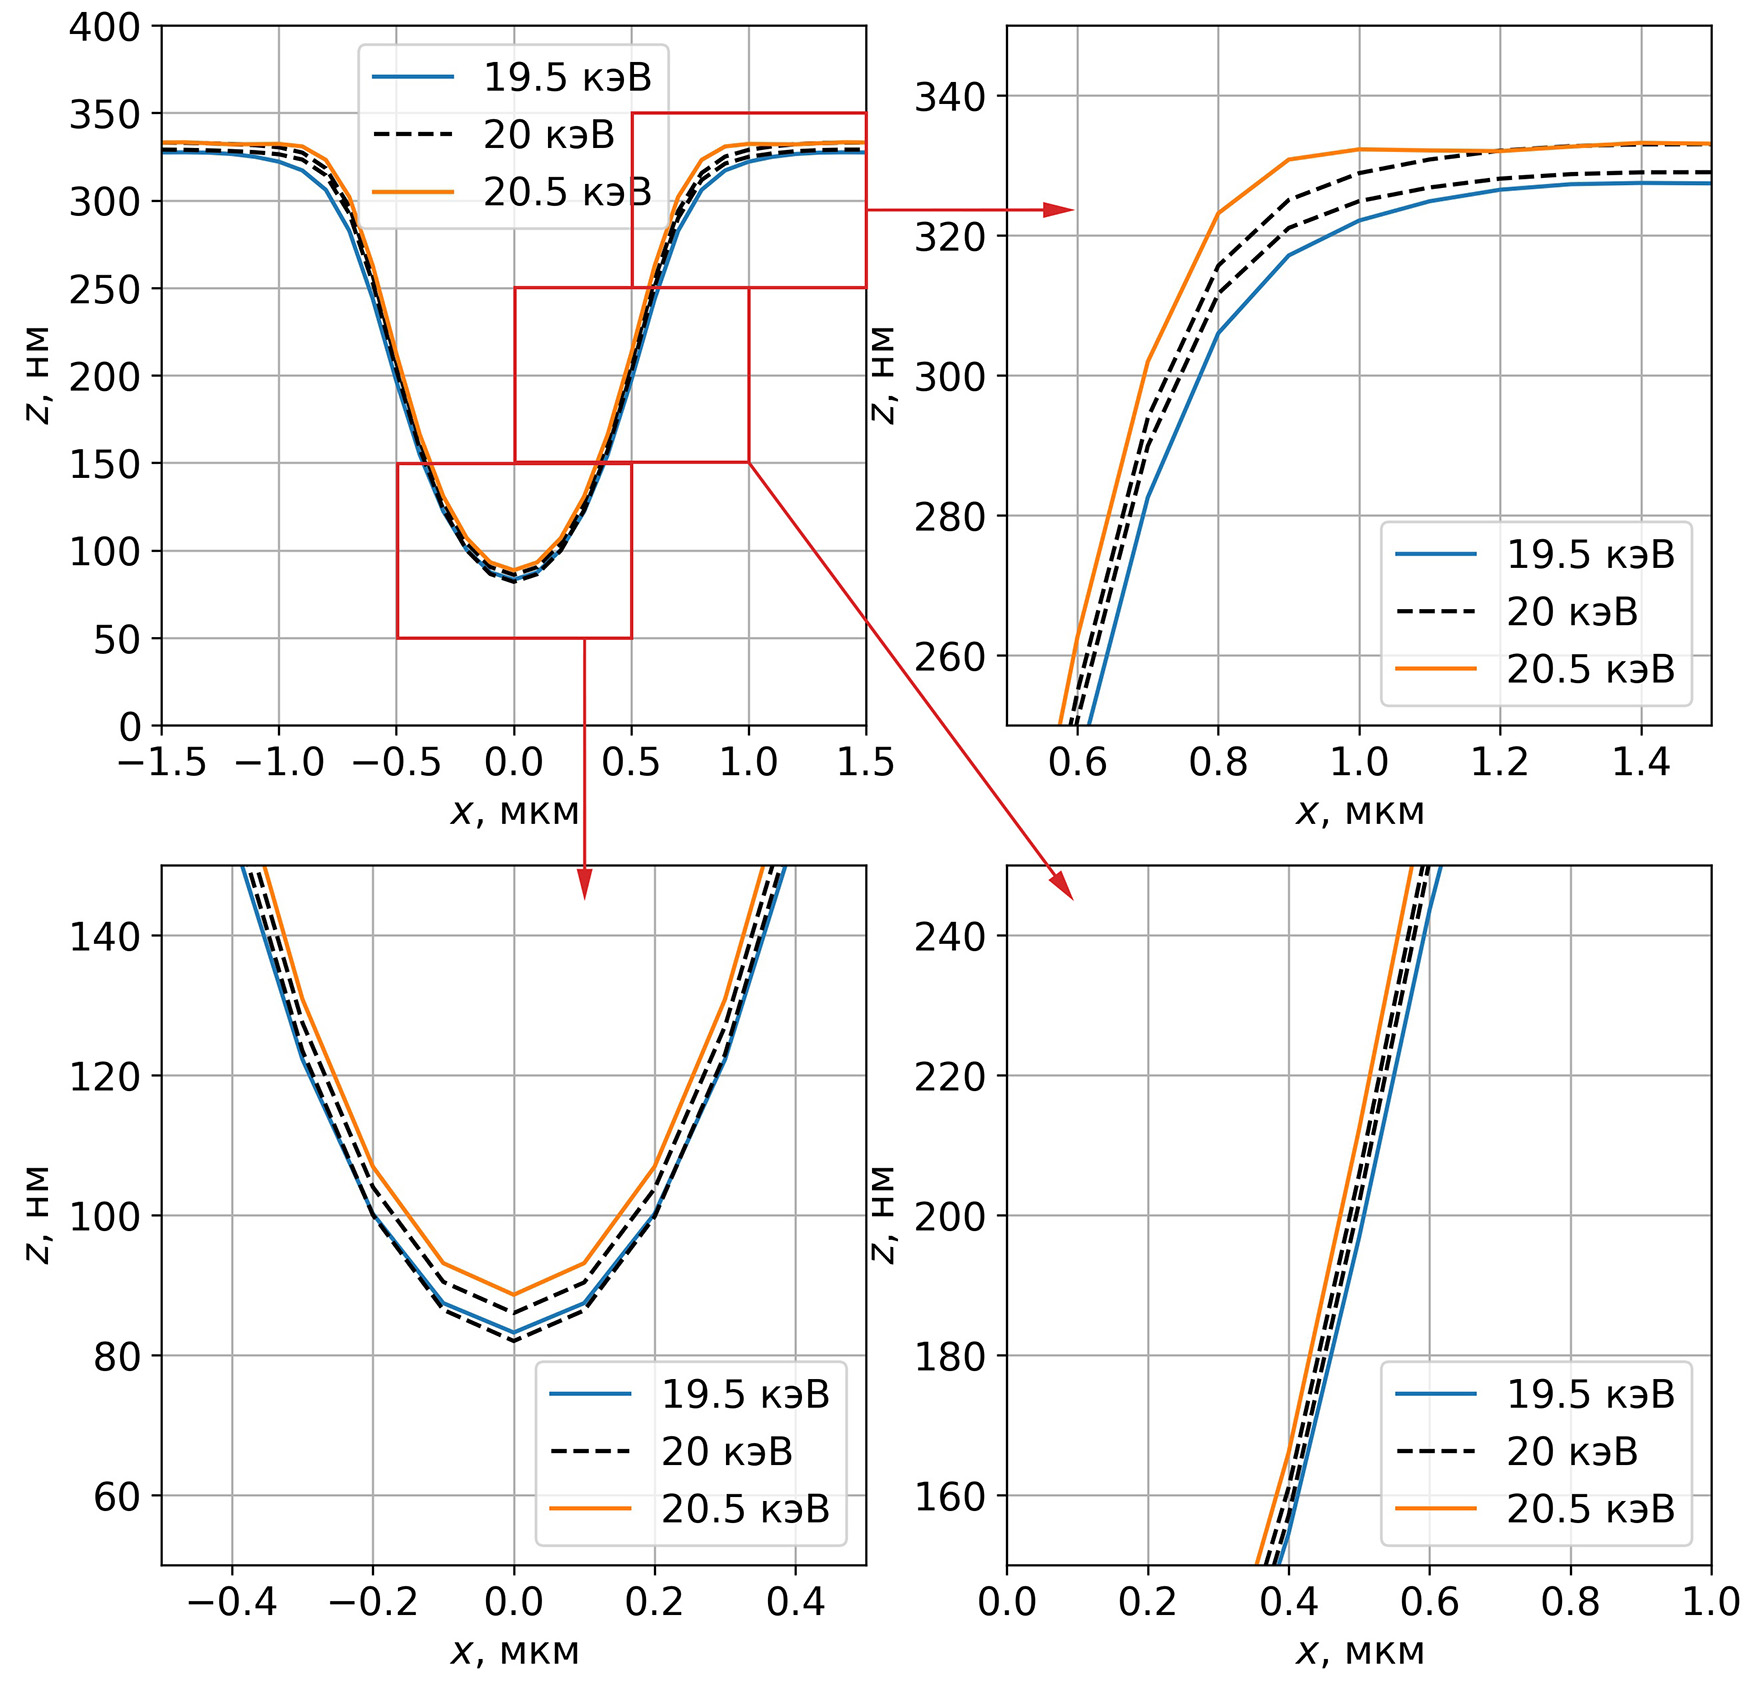
\includegraphics[width=\linewidth]{DEBER_stability/vary_E_4_arrows_200_CUT}
	\end{center}
%	\vspace{-1em}
	\caption{Изменения профиля линии, полученной методом СЭЛТР, вызванные отклонениями энергии пучка от исходного значения 20 кэВ при $T$~=~150~$^\circ$C, $t_\mathrm{exp}$ = 100 c и $I$ = 4.56 нА.}
%	\vspace{1em}
	\label{fig:DEBER_vary_E}
\end{figure}

\begin{figure}[h!]
	\begin{center}
		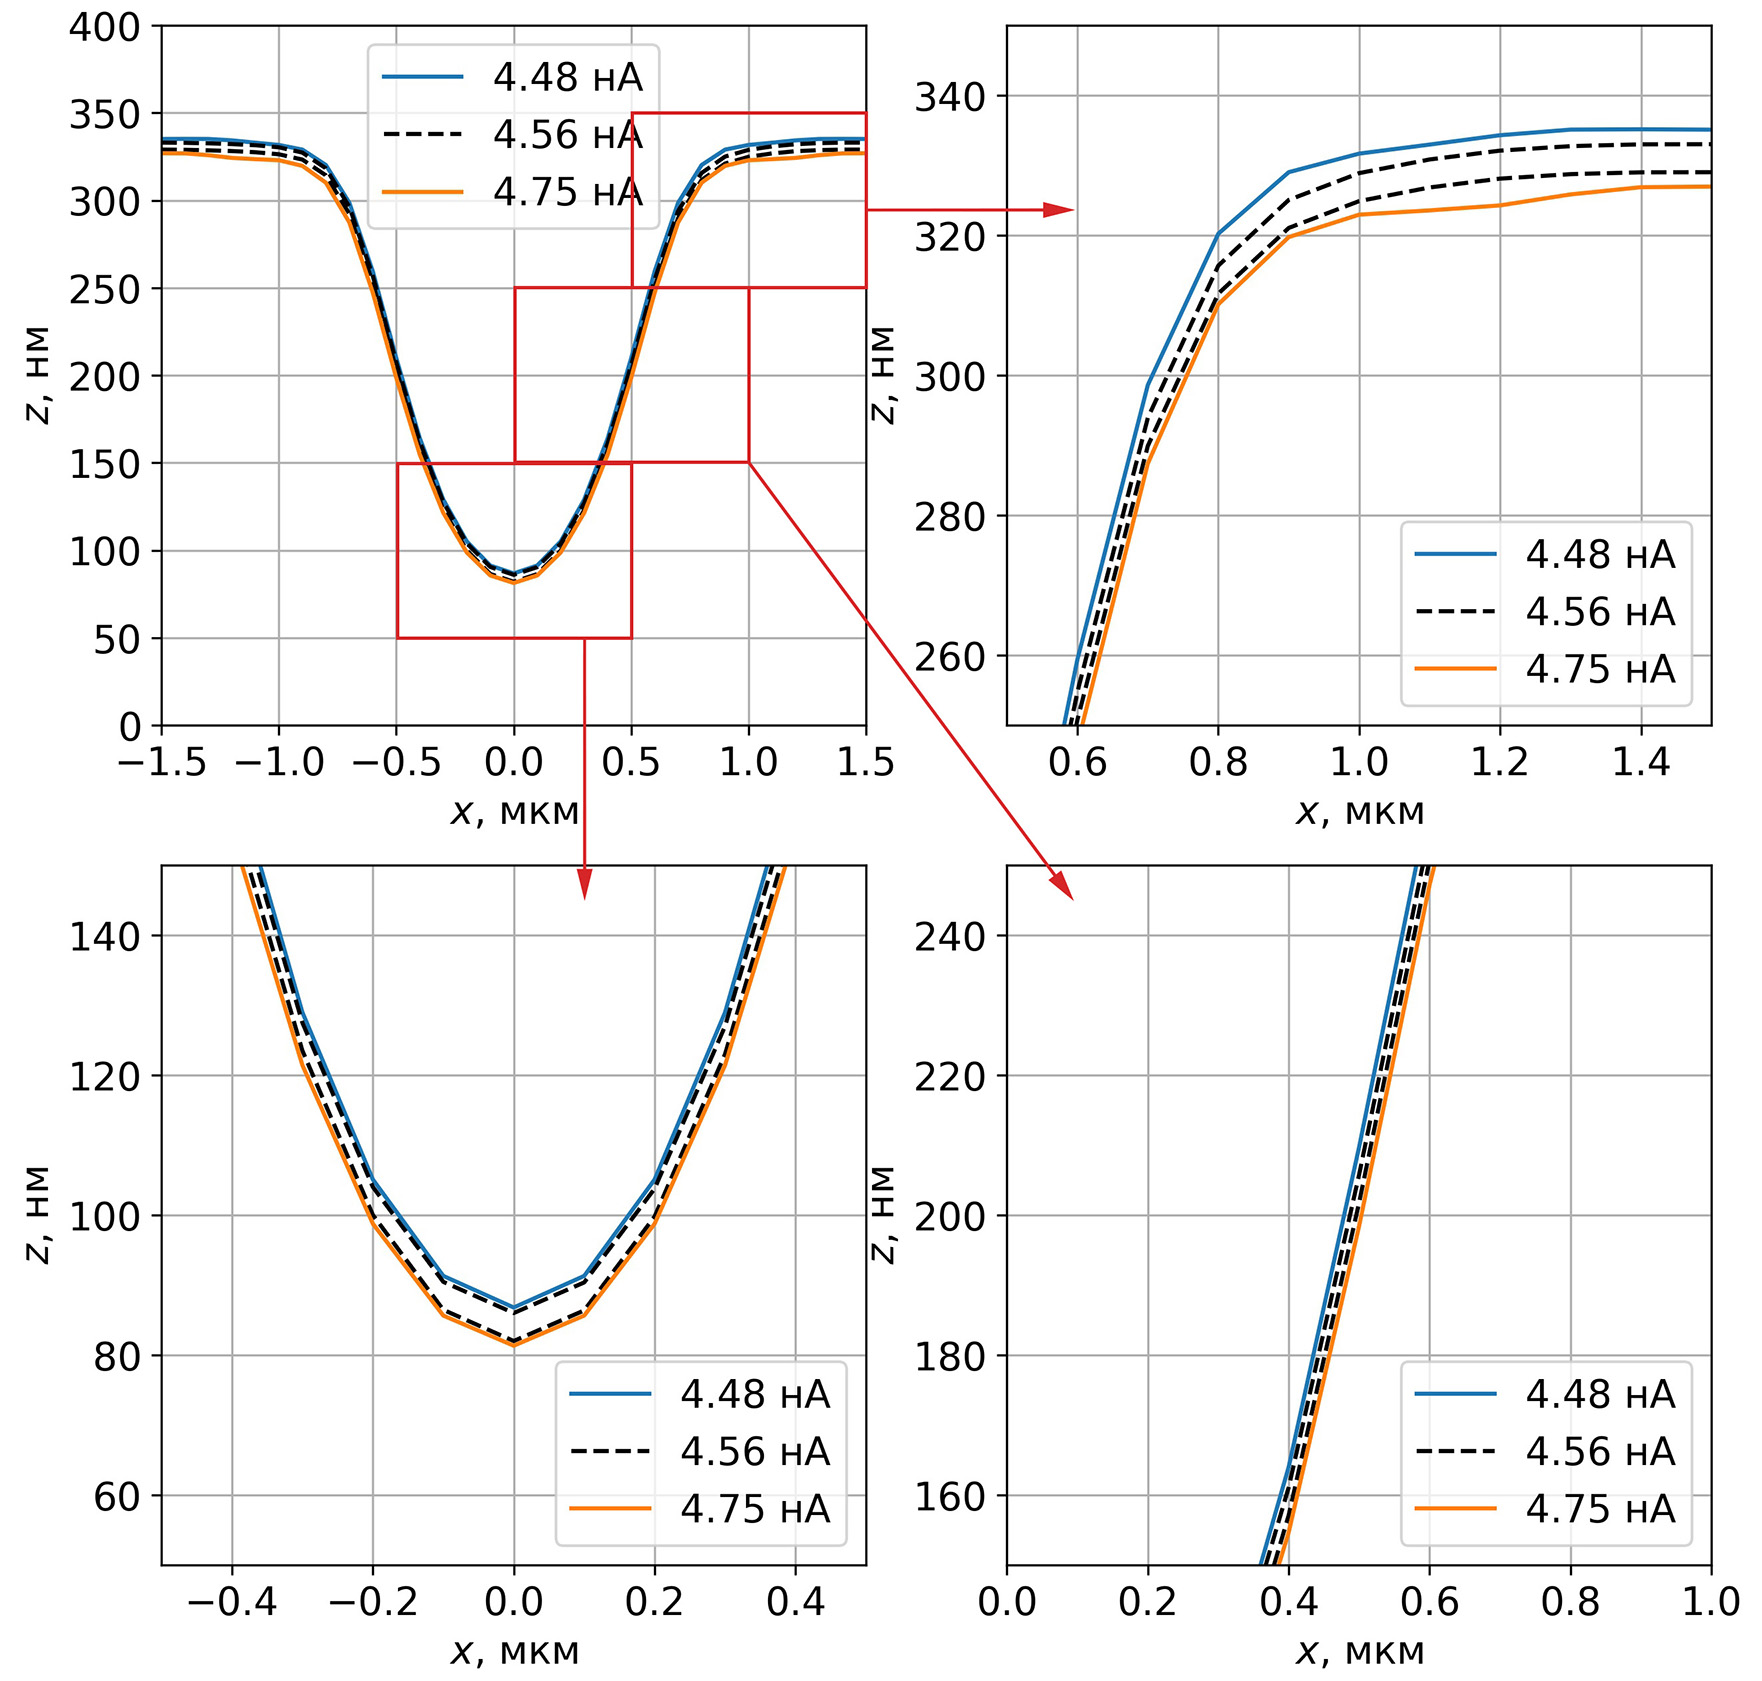
\includegraphics[width=\linewidth]{DEBER_stability/vary_I_4_arrows_200_CUT}
	\end{center}
%	\vspace{-1em}
	\caption{Изменения профиля линии, полученной методом СЭЛТР, вызванные отклонениями тока экспонирования от исходного значения 4.56 нА при $E$ = 20~кэВ, $T$ = 150~$^\circ$C и $t_\mathrm{exp}$ = 100 c.}
	\label{fig:DEBER_vary_I}
\end{figure}

\begin{figure}[h!]
	\begin{center}
		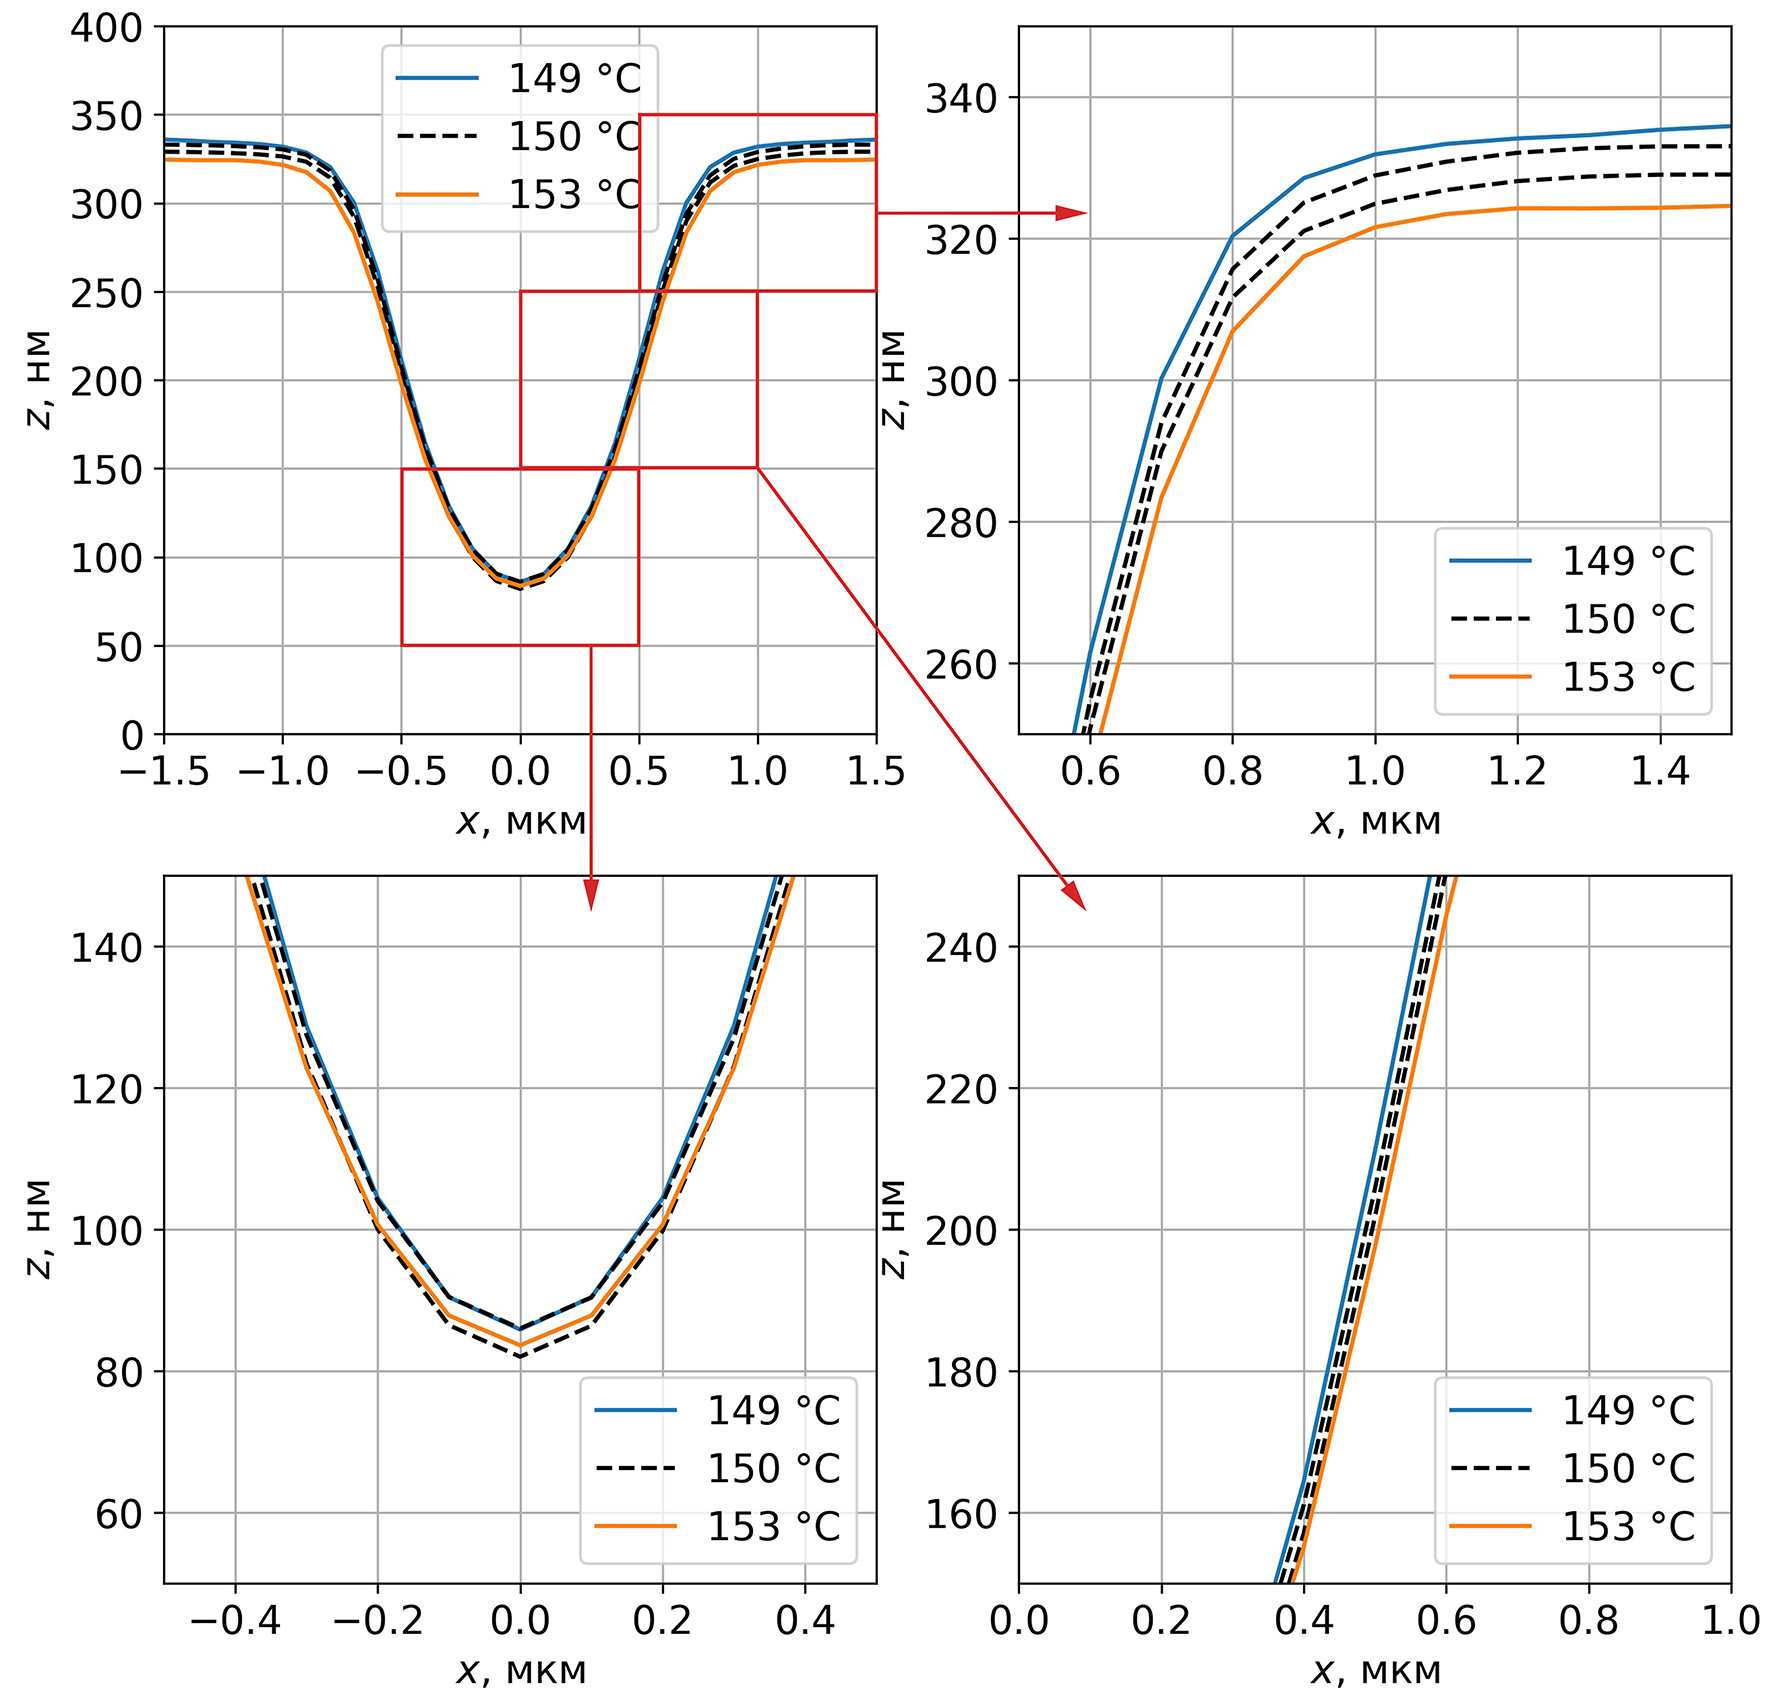
\includegraphics[width=\linewidth]{DEBER_stability/vary_T_4_arrows_200_CUT}
	\end{center}
	\vspace{-0.5em}
	\caption{Изменения профиля линии, полученной методом СЭЛТР, вызванные отклонениями температуры образца от исходного значения 150~$^\circ$C при $E$ =~20 кэВ, $t_\mathrm{exp}$ = 100 c и $I$ = 4.56 нА.}
	\label{fig:DEBER_vary_T}
	\vspace{0.5em}
\end{figure}

Как показано на рисунках~\ref{fig:DEBER_vary_E}, \ref{fig:DEBER_vary_I} и \ref{fig:DEBER_vary_T}, интервалы значений энергии пучка, тока экспонирования и температуры образца, при которых точки промоделированного профиля находятся в пределах 2 нм от исходного профиля, составляют примерно 19.5--20.5 кэВ, 4.48--5.75 нА и 149--153~$^\circ$C соответственно.
Таким образом, в качестве требований к стабильности параметров экспонирования в методе СЭЛТР могут быть приняты максимально допустимые значения флуктуаций энергии пучка, тока экспонирования и температуры образца, составляющие 0.5~кэВ, 0.1~нА и 1~$^\circ$C соответственно.

\section{Влияние скорости охлаждения образца на результирующий профиль}

Важной особенность метода СЭЛТР является тот факт, что формирование профиля завершается только при охлаждении образца до температуры около 80~$^\circ$C, что занимает некоторое время после окончания экспонирования.
В данном разделе приводятся результаты моделирования конечного профиля линии, получаемой методом СЭЛТР, при значениях скорости охлаждения образца, отличающихся от скорости его охлаждения в эксперименте.

Как и ранее, считалось, что экспонирование резиста в процессе СЭЛТР производится ``в кадр'' с параметрами кадра, описанными в разделе~\ref{sec:verification}.
В качестве исходных параметров экспонирования были приняты $T$ = 130~$^\circ$C, $t_\mathrm{exp}$~=~100~c, $I$ = 4.56 нА, диаметр пучка составлял 600 нм, начальная толщина слоя ПММА -- 500 нм, зависимость температуры образца от времени при охлаждении изначально описывалась экспериментальной кривой охлаждения, приведенной на рисунке~\ref{fig:exp_cooling} (профиль линии, получаемой в этих условиях, приведен на рисунке~\ref{fig:DEBER_4_profiles}в).
При данных параметрах процесса СЭЛТР в слое ПММА на момент остывания присутствуют микрополости, что обеспечивает меньший радиус кривизны профиля в центре линии по отношению к случаю полного заполнения микрополостей (рисунки~\ref{fig:DEBER_4_profiles}а, \ref{fig:DEBER_4_profiles}б и \ref{fig:DEBER_4_profiles}г).

На рисунке~\ref{fig:DEBER_cooling} приведены промоделированные профили линий, полученных методом СЭЛТР при одинаковых условиях экспонирования, описанных выше, но с разными значениями скорости охлаждения образца после экспонирования.
Результаты моделирования демонстрируют заметное влияние микрополостей в слое резиста на форму профиля, особенно в центре линии.
Исходя из того, что среднеквадратичное отклонение точек промоделированных профилей в центре линии при наличии микрополостей составляет около 15 нм, требование к стабильности скорости охлаждения образца может быть сведено к максимально допустимой флуктуации скорости охлаждения образца, равной 0.1~$^\circ$C/с (данное значение получено аналогично максимально допустимым значениям флуктуаций параметров экспонирования, приведенным ранее).

\begin{figure}[h]
	\begin{minipage}{0.48\textwidth}
		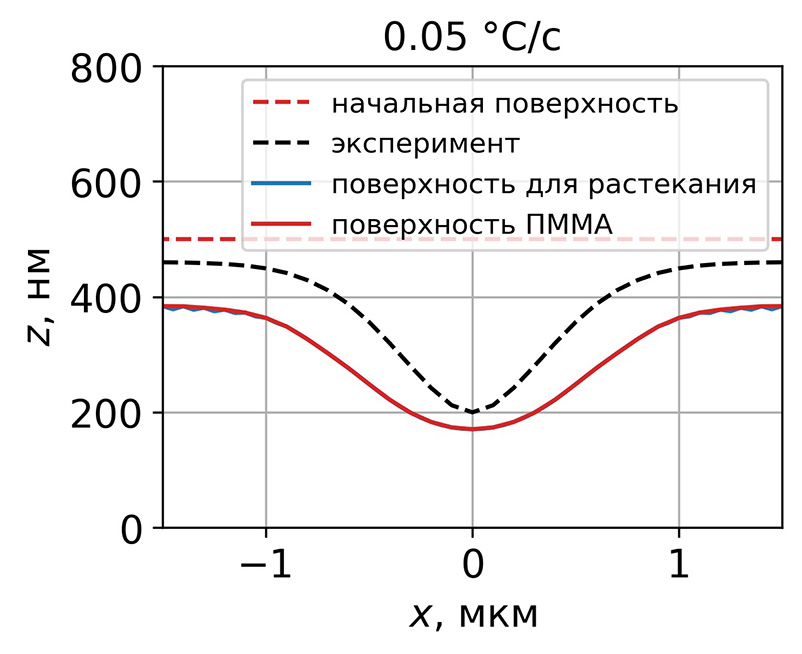
\includegraphics[width=\linewidth]{DEBER_cooling/cooling_0p05_200} \\
		\vspace{-13em} \\ \text{\hspace{0em} a}) \\ \vspace{13em}
	\end{minipage}
	\begin{minipage}{0.48\textwidth}
		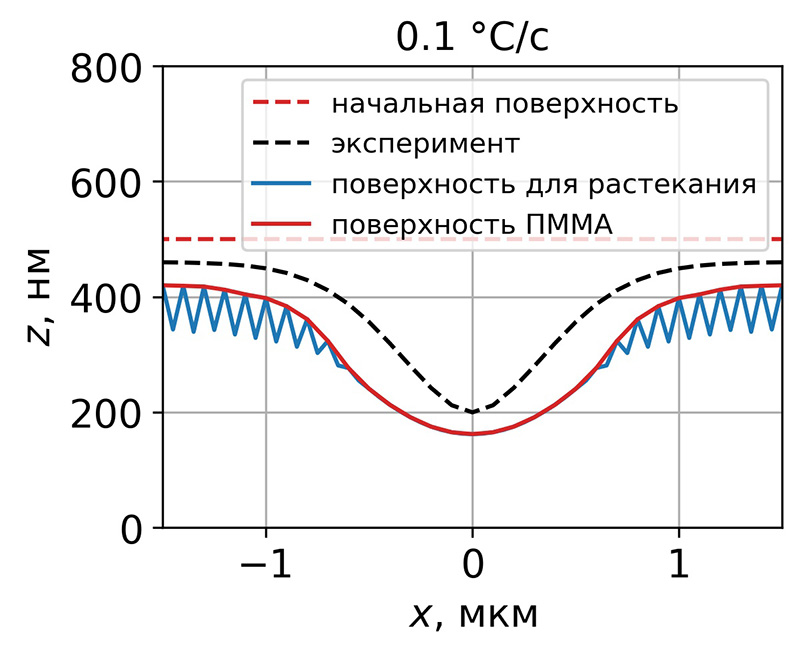
\includegraphics[width=\linewidth]{DEBER_cooling/cooling_0p1_200} \\
		\vspace{-13em} \\ \text{\hspace{-0.1em} б}) \\ \vspace{13em}
	\end{minipage}
	
	\vspace{-3em}
	
	\begin{minipage}{0.48\textwidth}
		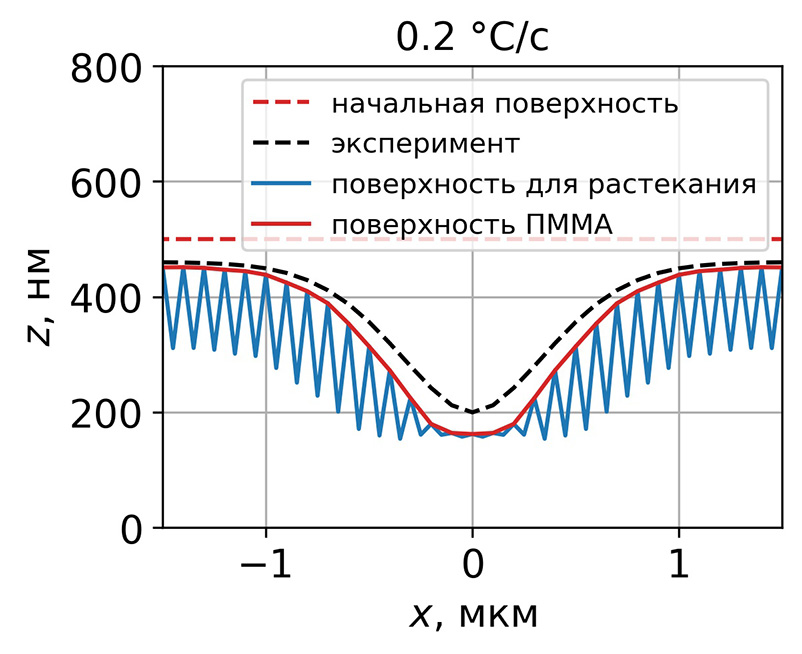
\includegraphics[width=\linewidth]{DEBER_cooling/cooling_0p2_200} \\
		\vspace{-13em} \\ \text{\hspace{0em} в}) \\ \vspace{13em}
	\end{minipage}
	\begin{minipage}{0.48\textwidth}
		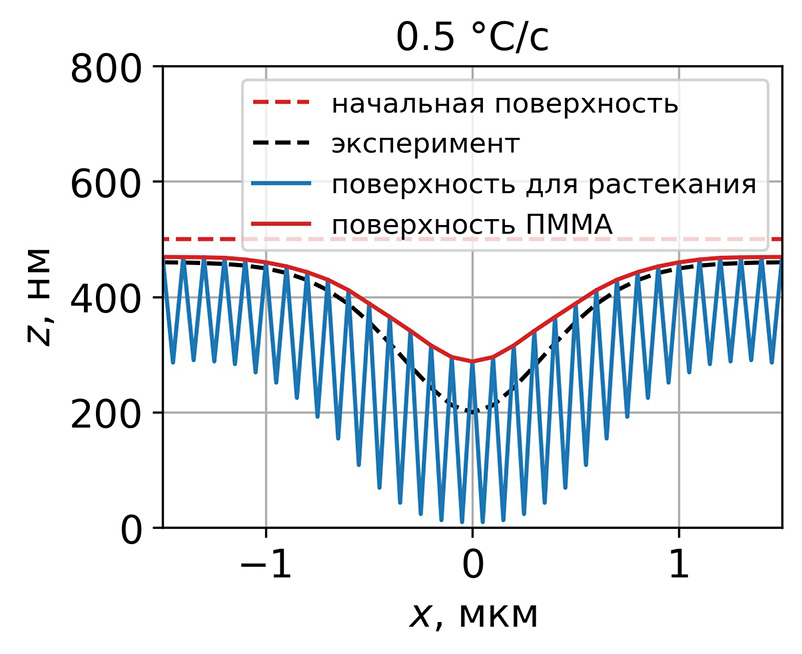
\includegraphics[width=\linewidth]{DEBER_cooling/cooling_0p5_200} \\
		\vspace{-13em} \\ \text{\hspace{-0.1em} г}) \\ \vspace{13em}
	\end{minipage}
	\vspace{-3em}
	\caption{Промоделированные профили, полученные методом СЭЛТР при $T$ = 130~$^\circ$C, $t_\mathrm{exp}$ = 100 c и $I$ = 4.56 нА. Скорость охлаждения образцов варьируется в пределах 0.05--0.5 $^\circ$C.}
	\label{fig:DEBER_cooling}
	\vspace{1em}
\end{figure}

\section{Применение метода сухого электронно-лучевого травления для формирования синусоидальных голографических решеток}

Проведенные эксперименты показали, что при экспонировании резиста в процессе СЭЛТР ``в кадр'' профиль получаемого рельефа имеет волнообразную форму.
Вследствие этого целесообразным является изучение возможности использования метода СЭЛТР для формирования синусоидальных голографических решеток, широко использующихся в оптике и получаемых в основном методом интерференционной литографии~\cite{Harrison2004_sin_gratings, Tishchenko2017_sin_gratings}.
Характерными параметрами таких решеток являются плотность штрихов порядка 1000 1/мм и глубина рельефа порядка 100 нм~\cite{Harvey2020_diffraction_gratings}.

Было проведено моделирование профиля рельефа, получаемого методом СЭЛТР при экспонировании ``в кадр'' c числом линий в кадре, равным 625, и отношением длины кадра к его ширине 1.3:1.
Расстояние между линиями варьировалось от 0.5 до 2 мкм, температура образца и ток экспонирования были приняты равными 150~$^\circ$C и 4.56 нА соответственно, начальная толщина слоя ПММА составляла 500 нм.
В свою очередь, диаметр пучка, время экспонирования и скорость охлаждения образца после экспонирования подбирались для получения профиля, максимально близкого к синусоидальному.
Результаты моделирования представлены на рисунках~\ref{fig:DEBER_holo_2um}, \ref{fig:DEBER_holo_1um} и \ref{fig:DEBER_holo_0p6um}.

На основании результатов моделирования можно заключить, что методом СЭЛТР могут быть получены синусоидальные голографические решетки с периодом до 0.5 мкм, что соответствует плотности штрихов 2000 1/мм.
Как показано на рисунке~\ref{fig:DEBER_holo_2um}, рельеф с синусоидальным профилем может быть получен как при полном или частичном наличии микрополостей в слое резиста (рисунки~\ref{fig:DEBER_holo_2um}a, ~\ref{fig:DEBER_holo_2um}б), так и при их отсутствии (рисунки~\ref{fig:DEBER_holo_2um}в, ~\ref{fig:DEBER_holo_2um}г).
При начальной толщине слоя ПММА, равной 500 нм, глубина рельефа может составлять от 0 до 200 нм в зависимости от концентрации микрополостей в слое ПММА.
При этом среднеквадратичное отклонение промоделированных профилей от графика функции синус составляет менее 5\% от глубины решетки.
Полученные в \linebreak ПММА синусоидальные решетки могут быть в дальнейшем покрыты металлом или перенесены в металл путем травления в реакторе индуктивно-связанной плазмы~\cite{Bruk_2016_mee}, что обеспечит формирование отражательной синусоидальной голографической решетки.

% 2 um
\begin{figure}[t!]
	\begin{minipage}{0.48\textwidth}
			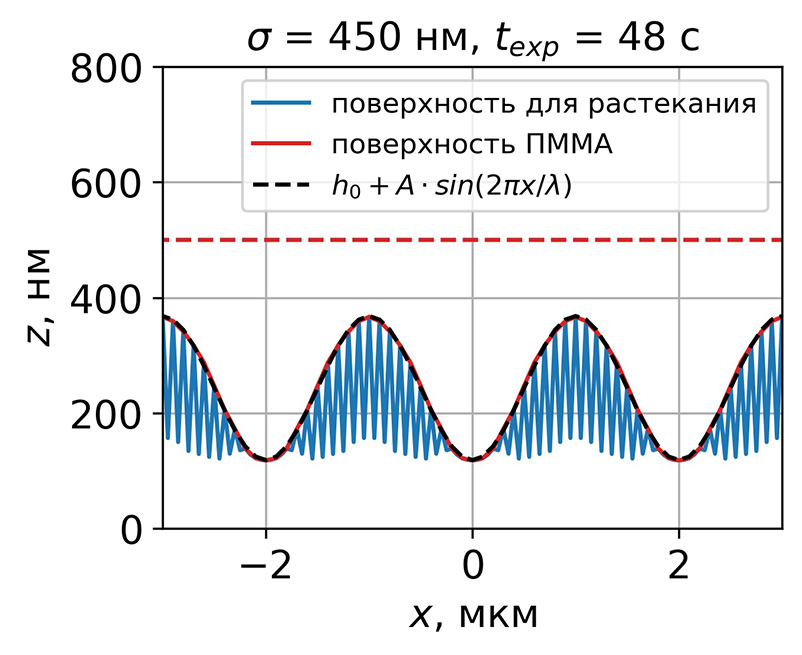
\includegraphics[width=\linewidth]{DEBER_holo/2_um/holo_1C_s450_48s_um_200} \\
			\vspace{-13em} \\ \text{\hspace{0em} a}) \\ \vspace{13em}
		\end{minipage}
	\begin{minipage}{0.48\textwidth}
			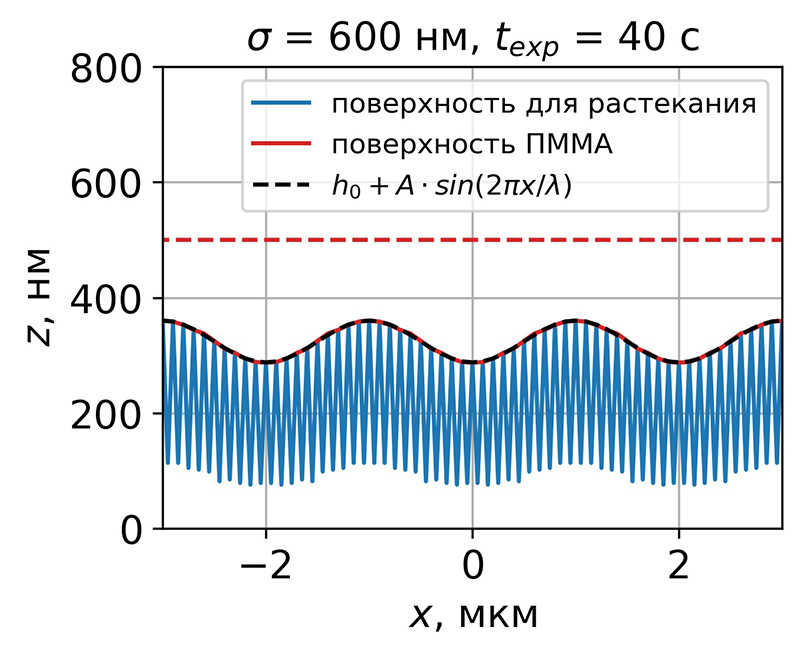
\includegraphics[width=\linewidth]{DEBER_holo/2_um/holo_1C_s600_40s_um_200} \\
			\vspace{-13em} \\ \text{\hspace{-0.1em} б}) \\ \vspace{13em}
		\end{minipage}
	
	\vspace{-3em}
	
	\begin{minipage}{0.48\textwidth}
			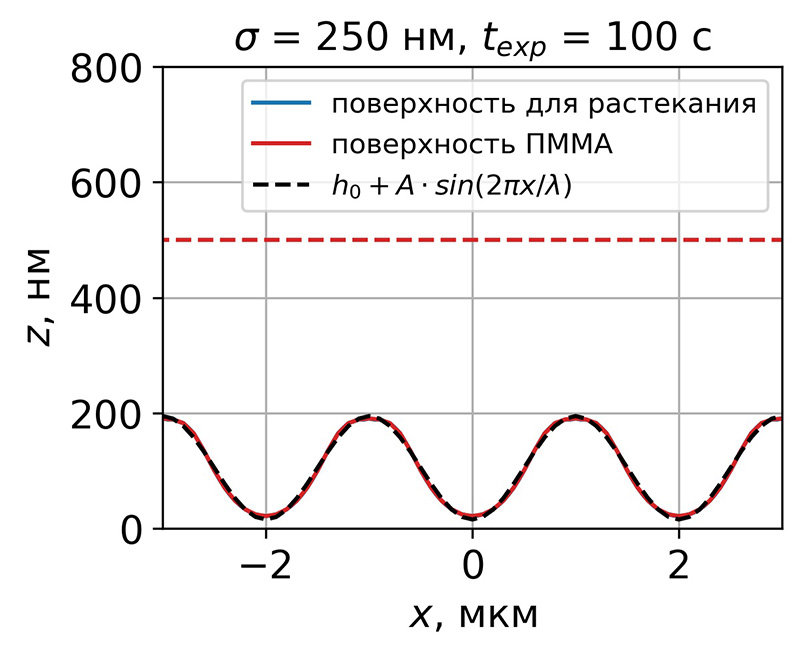
\includegraphics[width=\linewidth]{DEBER_holo/2_um//holo_10C_s250_100s_um_200} \\
			\vspace{-13em} \\ \text{\hspace{0em} в}) \\ \vspace{13em}
		\end{minipage}
	\begin{minipage}{0.48\textwidth}
			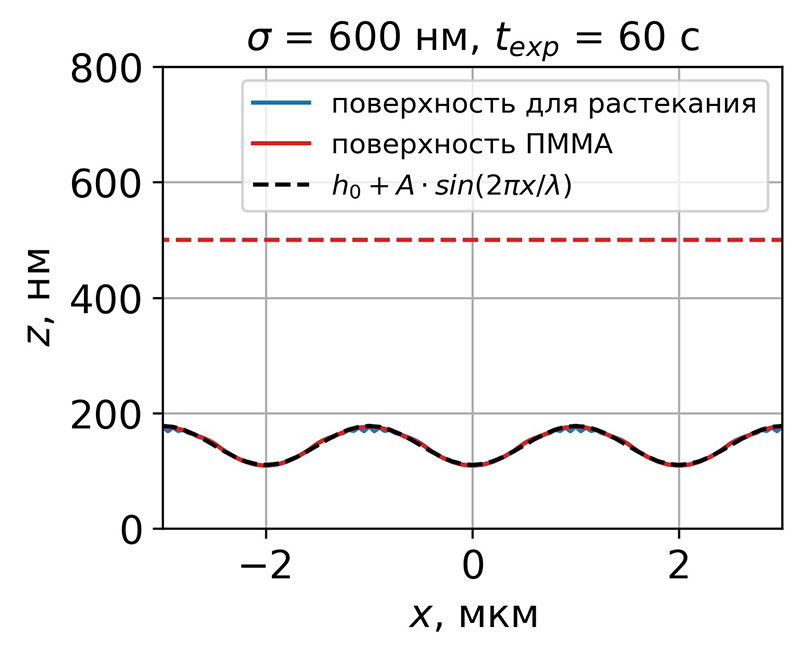
\includegraphics[width=\linewidth]{DEBER_holo/2_um/holo_1C_s600_60s_um_200} \\
			\vspace{-13em} \\ \text{\hspace{-0.1em} г}) \\ \vspace{13em}
		\end{minipage}
	\vspace{-3em}
	\caption{Промоделированные синусоидальные профили с пространственным периодом $\lambda$ = 2~мкм, полученные методом СЭЛТР в слое ПММА с начальной толщиной 500 нм. Температура образцов при экспонировании -- 150~$^\circ$C, ток экспонирования -- 4.56 нА, распределение плотности тока в пучке считается нормальным со среднеквадратичным отклонением $\sigma$. Значения $\sigma$ и $t_\mathrm{exp}$ были подобраны для получения синусоидального профиля. После экспонирования образец а) охлаждался со скоростью 10~$^\circ$C/с, образцы б)--г) -- со скоростью 1~$^\circ$C/с. Черная пунктирная линия обозначает аппроксимацию промоделированного профиля функцией синус.}
	\label{fig:DEBER_holo_2um}
\end{figure}


% 1 um
\begin{figure}[t!]
	\begin{minipage}{0.48\textwidth}
		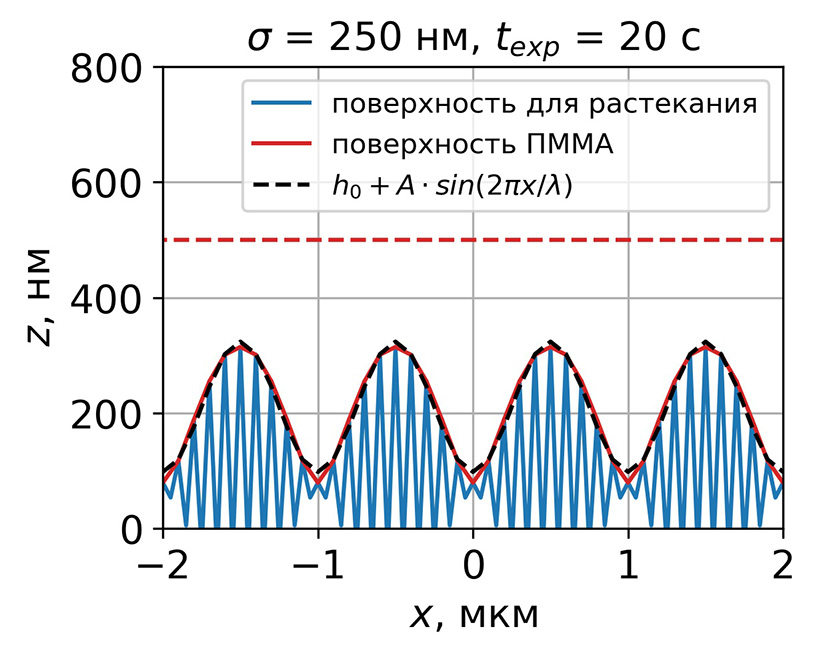
\includegraphics[width=\linewidth]{DEBER_holo/1_um/holo_1C_s250_20s_um_200} \\
		\vspace{-13em} \\ \text{\hspace{0em} a}) \\ \vspace{13em}
	\end{minipage}
	\begin{minipage}{0.48\textwidth}
		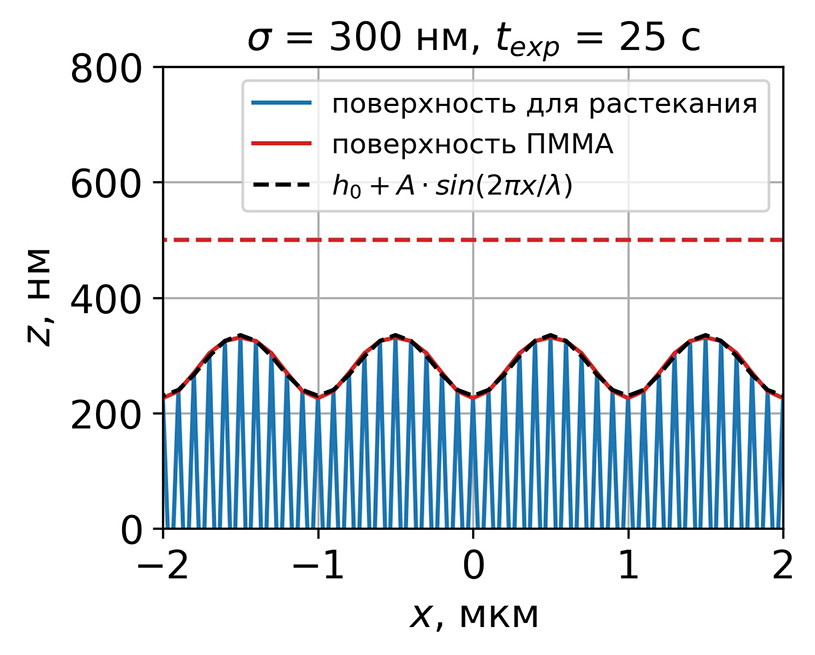
\includegraphics[width=\linewidth]{DEBER_holo/1_um/holo_5C_s300_25s_um_200} \\
		\vspace{-13em} \\ \text{\hspace{-0.1em} б}) \\ \vspace{13em}
	\end{minipage}
	\vspace{-3em}
	\caption{Промоделированные синусоидальные профили с пространственным периодом $\lambda$ = 1~мкм, полученные методом СЭЛТР в слое ПММА с начальной толщиной 500 нм. Температура образцов при экспонировании -- 150~$^\circ$C, ток экспонирования -- 4.56 нА, распределение плотности тока в пучке считается нормальным со среднеквадратичным отклонением $\sigma$. Значения $\sigma$ и $t_\mathrm{exp}$ были подобраны для получения синусоидального профиля. После экспонирования образец а) охлаждался со скоростью 1~$^\circ$C/с, образец б) -- со скоростью 5~$^\circ$C/с. Черная пунктирная линия обозначает аппроксимацию промоделированного профиля функцией синус.}
	\label{fig:DEBER_holo_1um}
\end{figure}


% 0.6 um
\begin{figure}[t!]
	\begin{minipage}{0.48\textwidth}
		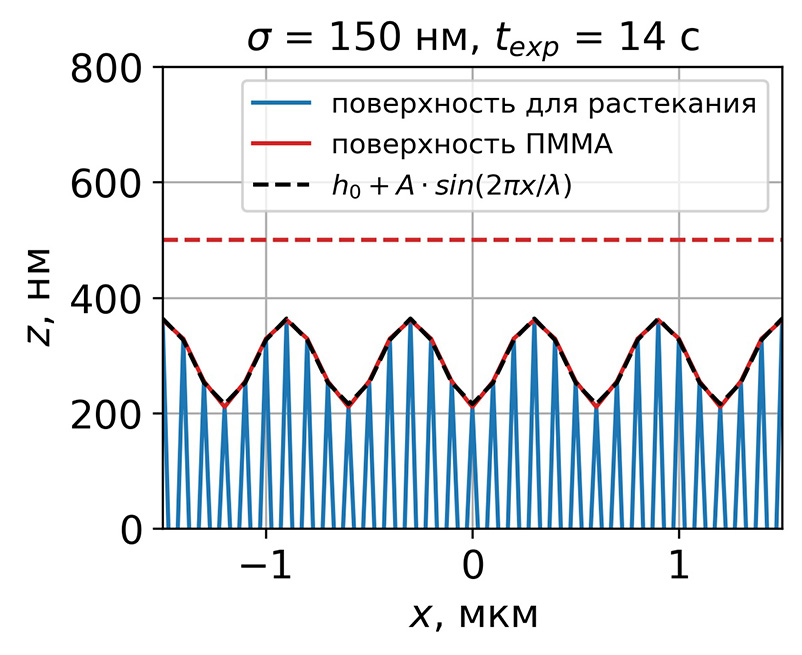
\includegraphics[width=\linewidth]{DEBER_holo/0p6_um/holo_10C_s150_14s_um_200} \\
		\vspace{-13em} \\ \text{\hspace{0em} a}) \\ \vspace{13em}
	\end{minipage}
	\begin{minipage}{0.48\textwidth}
		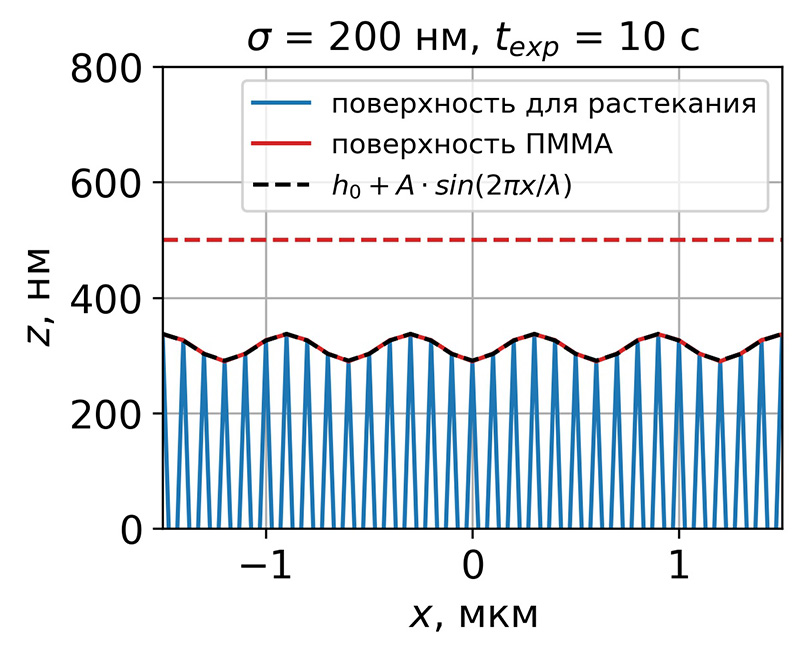
\includegraphics[width=\linewidth]{DEBER_holo/0p6_um/holo_2C_s200_10s_um_200} \\
		\vspace{-13em} \\ \text{\hspace{-0.1em} б}) \\ \vspace{13em}
	\end{minipage}
	
	\vspace{-3em}
	\caption{Промоделированные синусоидальные профили с пространственным периодом $\lambda$ = 0.6~мкм, полученные методом СЭЛТР в слое ПММА с начальной толщиной 500 нм. Температура образцов при экспонировании -- 150~$^\circ$C, ток экспонирования -- 4.56 нА, распределение плотности тока в пучке считается нормальным со среднеквадратичным отклонением $\sigma$. Значения $\sigma$ и $t_\mathrm{exp}$ были подобраны для получения синусоидального профиля. После экспонирования образец а) охлаждался со скоростью 10~$^\circ$C/с, образец б) -- со скоростью 2~$^\circ$C/с. Черная пунктирная линия обозначает аппроксимацию промоделированного профиля функцией синус.}
	\label{fig:DEBER_holo_0p6um}
	\vspace{2em}
\end{figure}

\section{Протекание сухого электронно-лучевого травления при экспонировании по произвольной области}

Приведенные выше промоделированные профили относятся к структурам, получаемым методом СЭЛТР при экспонировании вдоль серии параллельных линий либо вдоль одиночной линии.
Однако, при моделировании может быть заложено произвольное распределение плотности тока по области экспонирования.
Для демонстрации возможностей алгоритма были промоделированы профили, получаемые при экспонировании электронным лучом, плотность тока в котором описывается суммой двух (рисунки~\ref{fig:DEBER_multibeam}a, \ref{fig:DEBER_multibeam}б) или четырех (рисунки~\ref{fig:DEBER_multibeam}в, \ref{fig:DEBER_multibeam}г) функций Гаусса.
За счет этого разработанные в данной работе модель СЭЛТР и алгоритм моделирования профиля линии, получаемой в этом процессе, могут использоваться при определении параметров для формирования методом СЭЛТР необходимого профиля.
В самом деле, для получения методом СЭЛТР рельефа, профиль которого согласуется с предельным разрешением метода, параметры экспонирования и последующего охлаждения образца могут быть подобраны путем многократного моделирования конечного профиля с учетом выявленных особенностей метода.

\begin{figure}[t!]
	\begin{minipage}{0.48\textwidth}
%		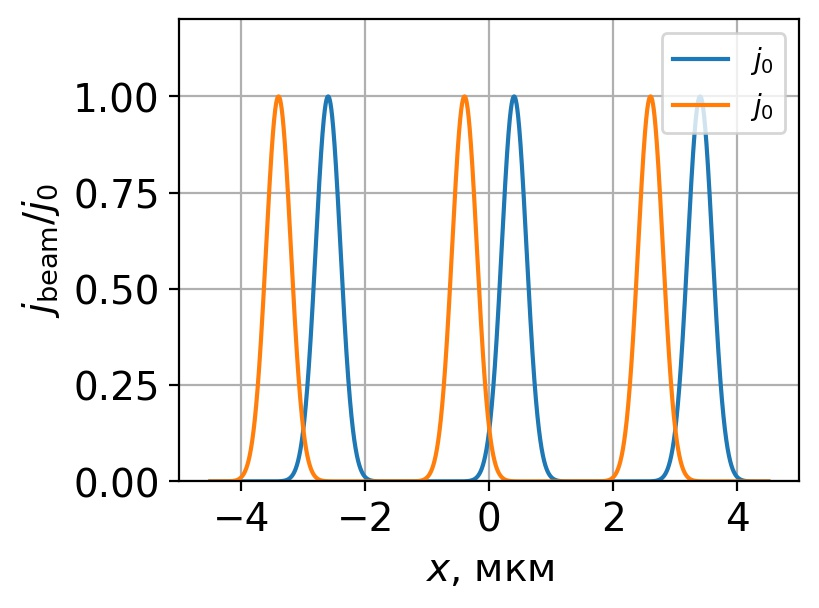
\includegraphics[width=\linewidth]{DEBER_asymmetric/pm_400_colors_200} \\
		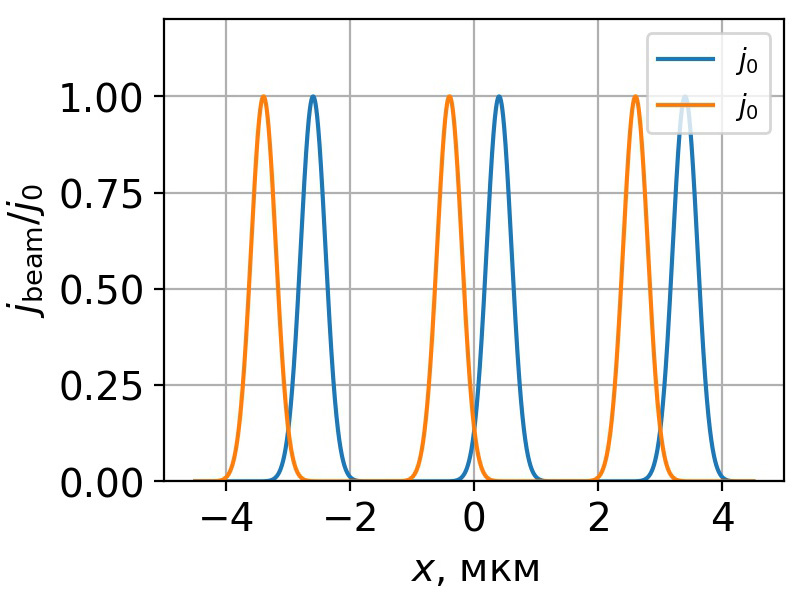
\includegraphics[width=\linewidth]{DEBER_asymmetric/pm_400_colors_200_cut} \\
		\vspace{-13em} \\ \text{\hspace{0em} a}) \\ \vspace{13em}
	\end{minipage}
	\begin{minipage}{0.48\textwidth}
		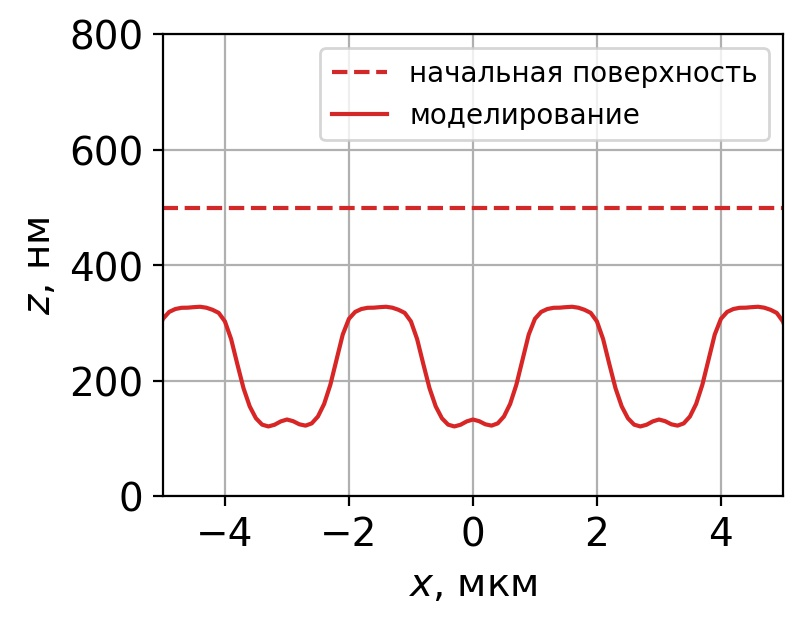
\includegraphics[width=\linewidth]{DEBER_asymmetric/pm_400_200} \\
		\vspace{-13em} \\ \text{\hspace{-0.1em} б}) \\ \vspace{13em}
	\end{minipage}
	
	\vspace{-3em}
	
	\begin{minipage}{0.48\textwidth}
		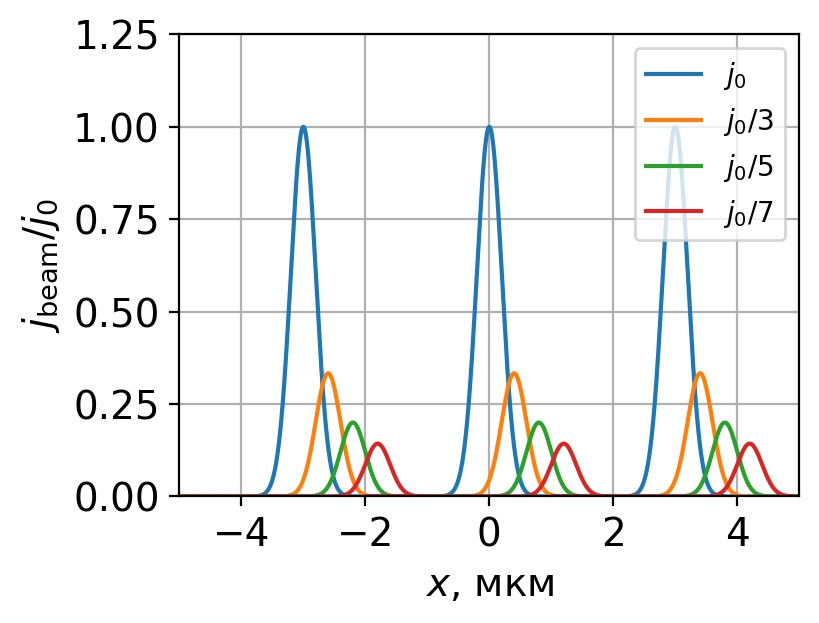
\includegraphics[width=\linewidth]{DEBER_asymmetric/asymmetric_beam_200} \\
		\vspace{-13em} \\ \text{\hspace{0em} в}) \\ \vspace{13em}
	\end{minipage}
	\begin{minipage}{0.48\textwidth}
		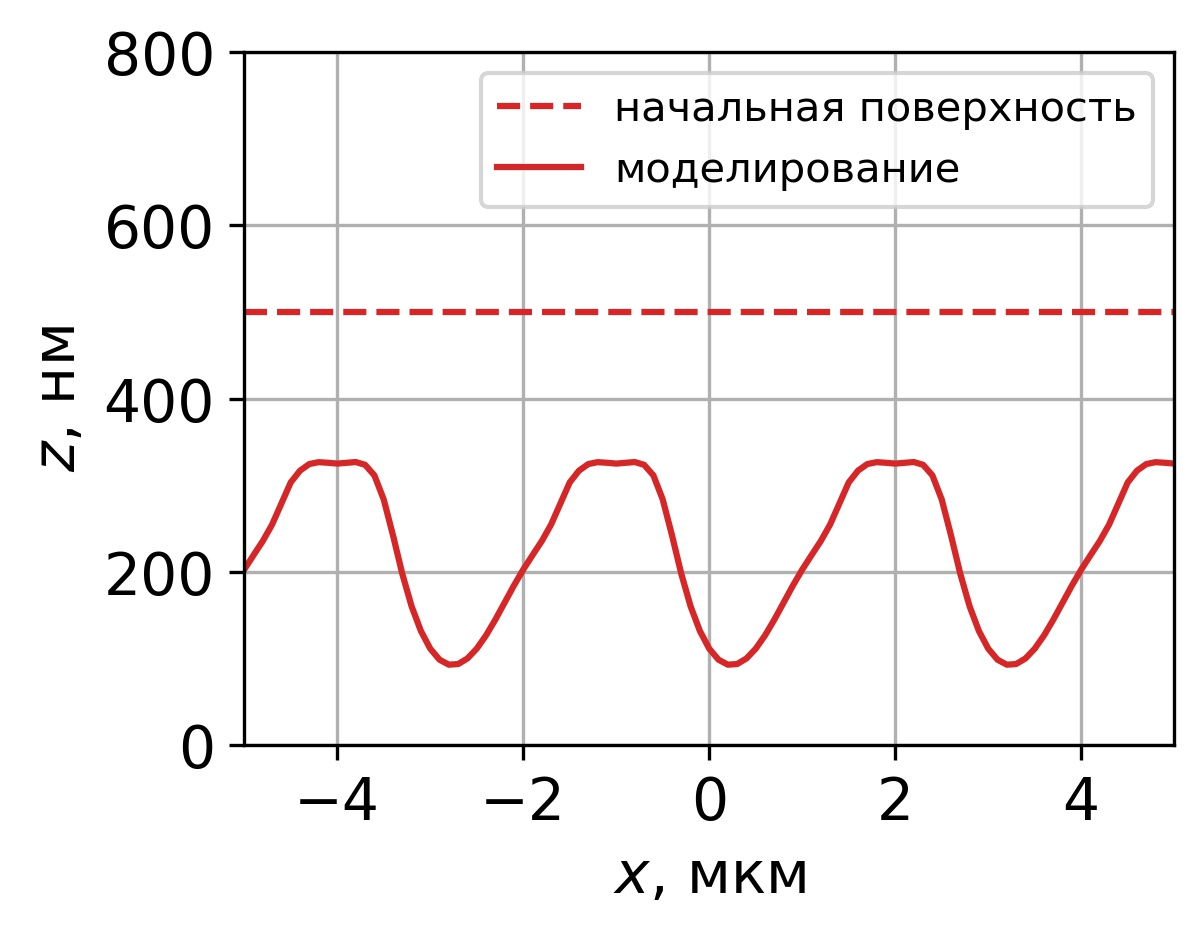
\includegraphics[width=\linewidth]{DEBER_asymmetric/asymmetric_profile_200} \\
		\vspace{-13em} \\ \text{\hspace{-0.1em} г}) \\ \vspace{13em}
	\end{minipage}
	\vspace{-3em}
	\caption{Промоделированные периодические профили с периодом 3~мкм, полученные в слое ПММА с начальной толщиной 500 нм методом СЭЛТР при экспонировании по области для двух различных распределений плотности тока в пучке. Температура резиста при экспонировании -- 150 $^\circ$C/с, время экспонирования -- 100 с, ток экспонирования -- 4.56 нА. Экспонирование резиста производится ``в кадр'' с параметрами кадра, описанными в разделе~\ref{sec:verification}. Охлаждение производится в соответствии с кривой охлаждения, приведенной на рисунке~\ref{fig:exp_cooling}.}
	\label{fig:DEBER_multibeam}
\end{figure}

\section{Выводы по главе}

В данной главе описывается верификация разработанной модели процесса СЭЛТР и приводятся результаты моделирования конечного профиля линий, получаемых методом СЭЛТР при различных параметрах процессов экспонирования и охлаждения образца. Резюмирую вышеизложенное, можно сделать следующие выводы:

\begin{itemize}
	\item Разработанная модель процесса СЭЛТР, учитывающая рассеяние электронного пучка, электронно-стимулированные разрывы молекул резиста, термическую деполимеризацию резиста и процессы растекания, позволяет с высокой точностью воспроизвести профиль линий, полученных в эксперименте.
	\item Микрополости, образующиеся в слое резиста за счет диффузии мономера, оказывают существенное влияние на профиль линии, получаемой методом СЭЛТР. Наличие микрополостей в центре линии на момент остывания обеспечивает меньший радиус кривизны профиля линии по отношению к тому случаю, когда микрополости на момент остывания отсутствуют.
	\item Максимально допустимые значения флуктуаций параметров экспонирования в процессе СЭЛТР, при которых возможно получение необходимого профиля, составляют около 0.5 кэВ, 0.1 нА и 1~$^\circ$C для энергии пучка, тока экспонирования и температуры образца соответственно.
	\item Формирование профиля линии в процессе СЭЛТР происходит не только на стадии экспонирования -- при охлаждении образца профиль линии продолжает формироваться за счет процессов растекания, что приводит к уменьшению глубины профиля и увеличению его ширины. Таким образом, для обеспечения высокого контраста получаемого изображения следует обеспечить как можно более высокую скорость охлаждения образца. При этом максимально допустимое значение флуктуации скорости охлаждения образца, при котором возможно получение необходимого профиля, составляет около 0.1~$^\circ$C/с.
	\item Для получения максимального латерального разрешения в методе СЭЛТР следует использовать узкий электронный пучок (шириной до 10~нм) с энергией от 25 кэВ. При этом также следует обеспечить высокую скорость охлаждения образца после экспонирования для предотвращения заполнения микрополостей на краях линии. В этом случае разрешение метода СЭЛТР и максимальный угол наклона стенок линии составят около 300 нм и 70$^\circ$ соответственно.
	\item Метод СЭЛТР может быть использован для получения синусоидальных голографических решеток с плотностью штрихов до 2000 1/мм.
	\item Разработанный алгоритм может быть использован для моделирования рельефа, получаемого методом СЭЛТР при экспонировании по произвольной области.
\end{itemize}

